\documentclass[hyperref={pdfpagelabels=false}]{beamer}
% beamer already loads hyperref; do NOT load \usepackage{hyperref} again.

\usepackage{ragged2e} % 文字向兩邊對齊
\renewcommand{\raggedright}{\leftskip=0pt \rightskip=0pt plus 0cm}

\usepackage{listings}
\usepackage{lmodern}
\usepackage{fontspec}
\usepackage{xeCJK}
\setCJKmainfont{Noto Sans CJK TC}
%（可選）若你會用到無襯線中文或等寬中文，建議補上：
\setCJKsansfont{Noto Sans CJK TC}
\setCJKmonofont{Noto Sans Mono CJK TC}

\usepackage[english]{babel}
\usepackage{amsmath,amssymb,amsfonts,amsthm}

% hyperref settings (since beamer already loads hyperref)
\hypersetup{
  colorlinks=true,
  urlcolor=blue,
  citecolor=blue,
  pdfborder={0 0 0}
}

\usepackage{accsupp}% http://ctan.org/pkg/accsupp
\newcommand{\emptyaccsupp}[1]{\BeginAccSupp{ActualText={}}#1\EndAccSupp{}}

\usepackage{tikz}
\usetikzlibrary{arrows,decorations.pathmorphing,backgrounds,fit,positioning,shapes.symbols,chains}

\usepackage{booktabs}
\usepackage{threeparttable}
\usepackage{colortbl} 
\usepackage{xcolor}
\usetikzlibrary{tikzmark}

\newcommand{\indep}{\perp\!\!\!\perp}
\newcommand{\nindep}{\not\!\perp\!\!\!\perp}

\beamertemplatefootpagenumber


\usepackage{listings}
%%%%%%%%%%%%%%%%%%%%%%%%%%%%%%%%%%%%%%%%%%%%%%%%%%%%%%%%%%%%%%%%%%%%%%%%%%%%%%
% LaTeX snippet: language and style definition of Stata for listings package.
%                [listings](http://www.ctan.org/pkg/listings) 
%                [Stata](http://www.stata.com/)
%
% Usage:
%     Copy the code into your preamble, or import it by `\include` .
%     then in your doc:
%     \lstinputlisting[style=numbers]{DO-SCRIPT}
%     \lstinputlisting[style=numbers, style=stata-editor]{DO-SCRIPT}
%     \lstinputlisting[style=nonumbers, frame=none]{DO-SCRIPT}
% How it works:
%     - The language is defined by `\lstdefinelanguage{Stata}`
%     - Four styles is defined by `\lstdefinestyle{STYLE-NAME}`, 
%       they are: numbers and no numbers, plain(black and white) and colorful
%       (colored roughly like stata editor.)
% Tips:
%     - Generally you only need to set your default in the last part,
%       that is, code inside of `\lstset`.
%     - Add more keywords(I can not list all of them) in the `\lstset` part.
%     - Do NOT leave any blank lines in commands
%       (`\lstddefinelanguage', `\lstdefinestyle` and `\lstset`)
%
% update: 2014-04-16
% version: 0.1
% author: kongs
% licence: MIT
% url: https://gist.github.com/kongs-sublime/10862838
%
% TODO: 
%       - finish keyword list.
%       - precise colors that match stata editor?
%       - make it flexible(fonts and style)
%
%%%%%%%%%%%%%%%%%%%%%%%%%%%%%%%%%%%%%%%%%%%%%%%%%%%%%%%%%%%%%%%%%%%%%%%%%%%%%%


% langugae defination
\lstdefinelanguage{Stata}{
	% Left for users to add missing commands,
	% with possibility of choosing different style.
	morekeywords=,
	% Popular add-on commands
	morekeywords=[2]{cntrade, chinafin, 
		wbopendata, spmap,
	},
	% System commands
	morekeywords=[3]{regress, summarize, 
		display,
	},
	% Keywords
	morekeywords=[4]{forvalues, if, foreach, set},
	% Built-in functions
	morekeywords=[5]{rnormal, runiform},
	morecomment=[l]{//},
	% morecomment=[l]{*},  // `*` maybe used as multiply operator. So use `//` as line comment.
	morecomment=[s]{/*}{*/},
	% morecomment=[s]{,}{//},
	% The following is used by macros, like `lags'.
	morecomment=[n][keywordstyle9]{`}{'},
	morestring=[b]",
	sensitive=true,
}

\lstdefinestyle{numbers}{
	numbers=left, 
	stepnumber=1, 
	numberstyle=\tiny\emptyaccsupp,
	xleftmargin=2em,
}

\lstdefinestyle{nonumbers}{
	numbers=none,
}

\lstdefinestyle{stata-plain}{
	language=Stata,
	basicstyle=\footnotesize\ttfamily,
}

\lstdefinestyle{stata-editor}{
	language=Stata,
	basicstyle=\footnotesize\ttfamily,  
	keywordstyle={\color{NavyBlue}},  
	keywordstyle=[2]{\color{NavyBlue}},
	keywordstyle=[3]{\color{NavyBlue}},
	keywordstyle=[4]{\color{NavyBlue}},
	keywordstyle=[5]{\color{Blue}},
	keywordstyle=[9]{\color{TealBlue}},
	stringstyle=\color{Maroon},
	commentstyle=\color{OliveGreen},
}

\lstset{
	language=Stata,
	style=stata-plain,
	% style=stata-editor,
	style=numbers,
	showstringspaces=false,
	breaklines,
	frame=single,
	% To add missing commands
	% morekeywords={xtreg, xtunitroot},
}




\title[]  
{Difference-in-Differences Design}


\author 
{Prof. Tzu-Ting Yang  \\ 楊子霆}

%\institute{Institute of Economics, Academia Sinica  \\ Econ, NTU}
\institute{Institute of Economics, Academia Sinica  \\ 中央研究院經濟研究所}
%\institute{Institute of Economics, Academia Sinica  \\ Econ, NTU}
%\institute{Institute of Economics, Academia Sinica  \\ IMES/IDAS, NCCU}

%\author 
%{楊子霆 \\ 中研院經濟所}

%\institute 
%{中正大學國際經濟專題研討}




\date
{\today}

\usetheme{CambridgeUS}
%\usecolortheme{seahorse}
\setbeamertemplate{footline}{%
	\hfill\usebeamercolor[fg]{page number in head/foot}%
	\usebeamerfont{page number in head/foot}%
	\insertframenumber\,/\,\inserttotalframenumber\hspace{1em}\vspace{2pt}%
}

% \usetheme{Boadilla}
% %\useinnertheme{rectangles}

% %\usetheme{CambridgeUS}
% \usecolortheme{seahorse}
% \setbeamertemplate{footline}{%
% 	\hfill\usebeamercolor[fg]{page number in head/foot}%
% 	\usebeamerfont{page number in head/foot}%
% 	\insertframenumber\,/\,\inserttotalframenumber\hspace{1em}\vspace{2pt}%
% }


% \usepackage{beamerthemeshadow}
% %\usecolortheme{seahorse}
% \setbeamertemplate{footline}{%
% 	\hfill\usebeamercolor[fg]{page number in head/foot}%
% 	\usebeamerfont{page number in head/foot}%
% 	\insertframenumber\,/\,\inserttotalframenumber\hspace{1em}\vspace{2pt}%
% }


%\usepackage{beamerthemeshadow}

\beamersetuncovermixins{\opaqueness<1>{25}}{\opaqueness<2->{15}}

\begin{document}
	
	
	\begin{frame}{}
	\titlepage
\end{frame}






\title[]  
{Causal Inference \\ Control-Based  v.s. Design-Based}


\author 
{}

%\institute{Institute of Economics, Academia Sinica  \\ Econ, NTU}
%\institute{Institute of Economics, Academia Sinica  \\ IMES/IDAS, NCCU}
\institute{}

%\author 
%{楊子霆 \\ 中研院經濟所}

%\institute 
%{中正大學國際經濟專題研討}




\date
{}


\begin{frame}{}
\titlepage
\end{frame}



\begin{frame}{Control-Based Causal Inference}

\begin{itemize}
\item So far, we have learned several control-based causal inference methods
\vspace{0.2cm}
\begin{itemize}
	\item Matching, regression, and causal machine learning
\end{itemize}
\vspace{0.2cm}
\item These methods are all based on CIA (\textbf{selection on observables}) 
\vspace{0.2cm}
\begin{itemize}
	\item Assumed all confounding factors can be observed
	\vspace{0.2cm}
	\item Thus, we can eliminate selection bias by comparing the treated and untreated units with the similar observed characteristics
\end{itemize}

%\item So far, we have learned several methods to deal with unobservable omitted variables

%\item In the next few weeks, we will go through some tools to deal with unobservable confounding factors

%\item We need more powerful tools or better data to eliminate selection bias from unobservable omitted variable 


\end{itemize}

\end{frame}





\begin{frame}{Unobservable Omitted Variable}

\begin{itemize}

\item If unobservabale confounding factors are time-invariant or common across units
\vspace{0.2cm}
\begin{itemize}
\item We can include \textbf{fixed effects} into regression to get causal effects
\end{itemize}
\vspace{0.2cm}
\item Yet, what if important confounding factors are unobserved and time-varying?

%\item So far, we have learned several methods to deal with unobservable omitted variables

%\item In the next few weeks, we will go through some tools to deal with unobservable confounding factors

%\item We need more powerful tools or better data to eliminate selection bias from unobservable omitted variable 


\end{itemize}

\end{frame}




\begin{frame}{Design-Based Causal Inference}

\begin{itemize}

\item Next four weeks, we will learn several methods to deal with unobservable omitted variables
\vspace{0.2cm}
\begin{itemize}
\item Difference-in-differences design
\vspace{0.2cm}
\item Synthetic control method 
	\vspace{0.2cm}
\item Instrumental variable design
\vspace{0.2cm}
\item Regression discontinuity design
	

\end{itemize}
\vspace{0.2cm}
\item The above methods utilize an exogenous factor that drives change in treatment status to estimate the causal effect		



%\item In the next few weeks, we will go through some tools to deal with unobservable confounding factors

%\item We need more powerful tools or better data to eliminate selection bias from unobservable omitted variable 


\end{itemize}

\end{frame}




\title[]  
{Main Idea}


\author 
{}

%\institute{Institute of Economics, Academia Sinica  \\ Econ, NTU}
%\institute{Institute of Economics, Academia Sinica  \\ IMES/IDAS, NCCU}
\institute{}

%\author 
%{楊子霆 \\ 中研院經濟所}

%\institute 
%{中正大學國際經濟專題研討}




\date
{}


\begin{frame}{}
	\titlepage
\end{frame}




\begin{frame}{Difference-in-Differences Design}{Main Idea}
	\begin{itemize}
		
		\item If we can observe \textbf{group-level} outcomes at multiple time points,
		\vspace{0.2cm}
		\begin{itemize}
			\item Especially before and after the treatment,
		\end{itemize}
		\vspace{0.2cm}
		
		\item And if we assume that, \textbf{in the absence of treatment}, the outcomes of the treatment and control groups would have followed \textbf{parallel trends},
		\vspace{0.2cm}
		
		\item Then we can construct the \textbf{counterfactual trend for the treatment group} using
		\vspace{0.2cm}
		\begin{itemize}
			\item The \textbf{observed trend in the control group}.
		\end{itemize}
		\vspace{0.2cm}
		
		\item By comparing the observed trend in the treatment group with its counterfactual trend, we can estimate the \textbf{causal effect of the treatment}.
		
	\end{itemize}
\end{frame}



\begin{frame}{Main Idea}{Graph}
	\begin{figure}
		\begin{tikzpicture}[comment/.style={rectangle, text centered}]
			\centering
			\draw [thick] (-0.5,0) -- (6,0) node[anchor=north west] {time};
			\draw [thick] (0,-0.5) -- (0,5) node[anchor=south east, xshift=-0.6cm](Y) {$Y$};
			\node [comment, below of = Y, yshift=0.3cm] {(outcome)};
			
			\draw [thick] (2.5,-0.5) -- (2.5,5);
			
			%\draw [thick] (0.5,0.5) -- (5.5,2) node[anchor=north west, yshift=0.2cm] {$D=0$};
			\draw [thick] (0.5,1.5) -- (2.5,2.1);
			\draw [thick] (2.5,2.1) -- (5.5,4.5) node[anchor=north west, yshift=0.3cm] {$D=1$};
			\draw [thick,dashed, white] (2.5,2.1) -- (5.5,3);
			
			\draw [thick,<->, white] (5,2.95) -- (5,4) node[anchor=west, yshift=-0.5cm] {DID estimate};
			
			\draw (1.3,0)--(1.3,0) node (1.3_0) {};
			\node [comment, below of = 1.3_0, yshift=0.5cm] {pre};
			
			\draw (4,0)--(4,0) node (4_0) {};
			\node [comment, below of = 4_0, yshift=0.5cm] {post};
			
		\end{tikzpicture}
	\end{figure}
\end{frame}








\begin{frame}{Main Idea}{Graph}
\begin{figure}
\begin{tikzpicture}[comment/.style={rectangle, text centered}]
\centering
\draw [thick] (-0.5,0) -- (6,0) node[anchor=north west] {time};
\draw [thick] (0,-0.5) -- (0,5) node[anchor=south east, xshift=-0.6cm](Y) {$Y$};
\node [comment, below of = Y, yshift=0.3cm] {(outcome)};

\draw [thick] (2.5,-0.5) -- (2.5,5);

\draw [thick] (0.5,0.5) -- (5.5,2) node[anchor=north west, yshift=0.2cm] {$D=0$};
\draw [thick] (0.5,1.5) -- (2.5,2.1);
\draw [thick] (2.5,2.1) -- (5.5,4.5) node[anchor=north west, yshift=0.3cm] {$D=1$};
\draw [thick,dashed, white] (2.5,2.1) -- (5.5,3);

\draw [thick,<->, white] (5,2.95) -- (5,4) node[anchor=west, yshift=-0.5cm] {DID estimate};

\draw (1.3,0)--(1.3,0) node (1.3_0) {};
\node [comment, below of = 1.3_0, yshift=0.5cm] {pre};

\draw (4,0)--(4,0) node (4_0) {};
\node [comment, below of = 4_0, yshift=0.5cm] {post};

\end{tikzpicture}
\end{figure}
\end{frame}





\begin{frame}{Main Idea}{Graph}
\begin{figure}
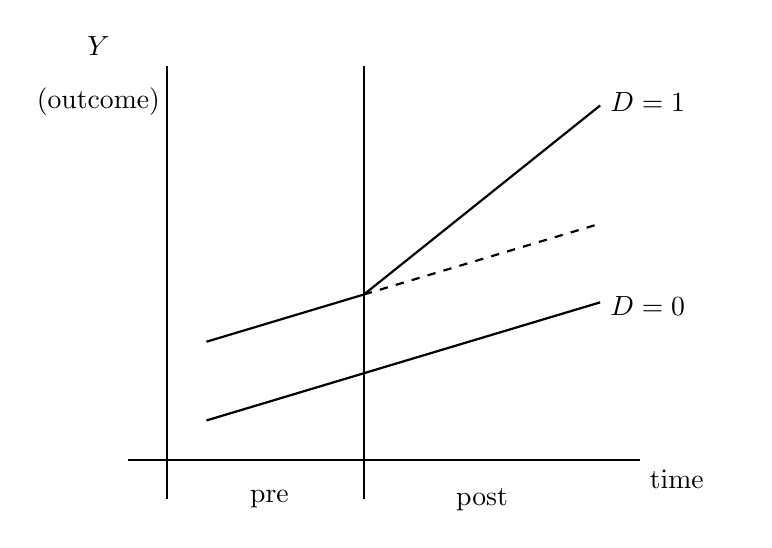
\begin{tikzpicture}[comment/.style={rectangle, text centered}]
\centering
\draw [thick] (-0.5,0) -- (6,0) node[anchor=north west] {time};
\draw [thick] (0,-0.5) -- (0,5) node[anchor=south east, xshift=-0.6cm](Y) {$Y$};
\node [comment, below of = Y, yshift=0.3cm] {(outcome)};

\draw [thick] (2.5,-0.5) -- (2.5,5);

\draw [thick] (0.5,0.5) -- (5.5,2) node[anchor=north west, yshift=0.2cm] {$D=0$};
\draw [thick] (0.5,1.5) -- (2.5,2.1);
\draw [thick] (2.5,2.1) -- (5.5,4.5) node[anchor=north west, yshift=0.3cm] {$D=1$};
\draw [thick,dashed] (2.5,2.1) -- (5.5,3);

\draw [thick,<->, white] (5,2.95) -- (5,4) node[anchor=west, yshift=-0.5cm] {DID estimate};

\draw (1.3,0)--(1.3,0) node (1.3_0) {};
\node [comment, below of = 1.3_0, yshift=0.5cm] {pre};

\draw (4,0)--(4,0) node (4_0) {};
\node [comment, below of = 4_0, yshift=0.5cm] {post};

\end{tikzpicture}
\end{figure}
\end{frame}


\begin{frame}{Main Idea}{Graph}
\begin{figure}
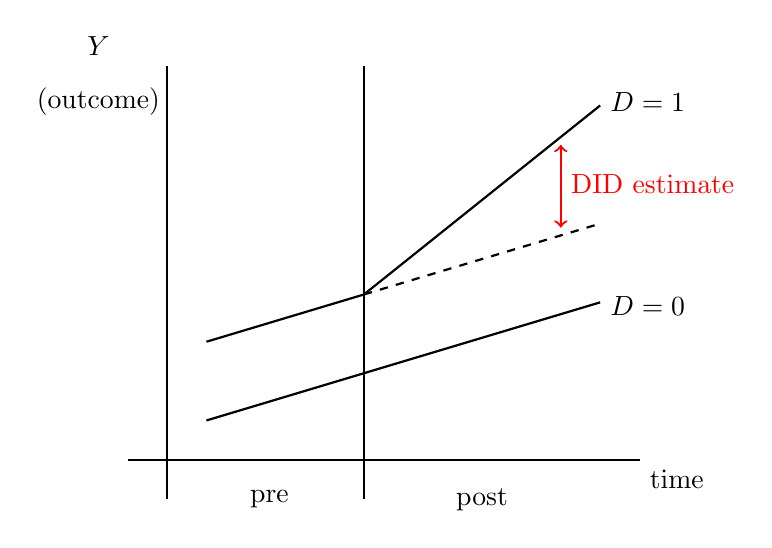
\begin{tikzpicture}[comment/.style={rectangle, text centered}]
\centering
\draw [thick] (-0.5,0) -- (6,0) node[anchor=north west] {time};
\draw [thick] (0,-0.5) -- (0,5) node[anchor=south east, xshift=-0.6cm](Y) {$Y$};
\node [comment, below of = Y, yshift=0.3cm] {(outcome)};

\draw [thick] (2.5,-0.5) -- (2.5,5);

\draw [thick] (0.5,0.5) -- (5.5,2) node[anchor=north west, yshift=0.2cm] {$D=0$};
\draw [thick] (0.5,1.5) -- (2.5,2.1);
\draw [thick] (2.5,2.1) -- (5.5,4.5) node[anchor=north west, yshift=0.3cm] {$D=1$};
\draw [thick,dashed] (2.5,2.1) -- (5.5,3);

\draw [thick,<->, red] (5,2.95) -- (5,4) node[anchor=west, yshift=-0.5cm] {DID estimate};

\draw (1.3,0)--(1.3,0) node (1.3_0) {};
\node [comment, below of = 1.3_0, yshift=0.5cm] {pre};

\draw (4,0)--(4,0) node (4_0) {};
\node [comment, below of = 4_0, yshift=0.5cm] {post};

\end{tikzpicture}
\end{figure}
\end{frame}






\begin{frame}{Main Idea}{Graph}
\begin{figure}
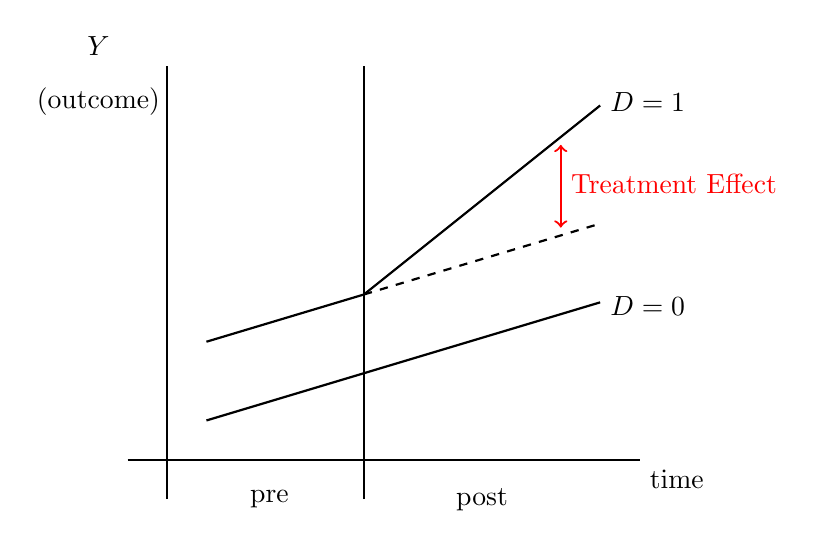
\begin{tikzpicture}[comment/.style={rectangle, text centered}]
\centering
\draw [thick] (-0.5,0) -- (6,0) node[anchor=north west] {time};
\draw [thick] (0,-0.5) -- (0,5) node[anchor=south east, xshift=-0.6cm](Y) {$Y$};
\node [comment, below of = Y, yshift=0.3cm] {(outcome)};

\draw [thick] (2.5,-0.5) -- (2.5,5);

\draw [thick] (0.5,0.5) -- (5.5,2) node[anchor=north west, yshift=0.2cm] {$D=0$};
\draw [thick] (0.5,1.5) -- (2.5,2.1);
\draw [thick] (2.5,2.1) -- (5.5,4.5) node[anchor=north west, yshift=0.3cm] {$D=1$};
\draw [thick,dashed] (2.5,2.1) -- (5.5,3);

\draw [thick,<->, red] (5,2.95) -- (5,4) node[anchor=west, yshift=-0.5cm] {Treatment Effect};

\draw (1.3,0)--(1.3,0) node (1.3_0) {};
\node [comment, below of = 1.3_0, yshift=0.5cm] {pre};

\draw (4,0)--(4,0) node (4_0) {};
\node [comment, below of = 4_0, yshift=0.5cm] {post};

\end{tikzpicture}
\end{figure}
\end{frame}




\begin{frame}{A Motivating Example}{Card \& Krueger (1994)}

 David Card and Alan B. Krueger (1994) ``\textbf{Minimum Wages and Employment: A Case Study of the Fast-Food Industry in New Jersey and Pennsylvania}" AER	
	\vspace{0.2cm}
\begin{itemize} 
\item They want to estimate the causal effect of raising minimum wage on employment of low-skilled workers
\end{itemize}
\end{frame}



\begin{frame}{A Motivating Example}{Card \& Krueger (1994)}

\begin{itemize} 
\item What is the effect of increasing the minimum wage on employment?
\vspace{0.2cm} 
\item Minimum wage is effective only in certain jobs: 
\vspace{0.2cm} 
\begin{itemize} 
\item Low-skilled jobs
\end{itemize}
\vspace{0.2cm} 
\item How much does an increase in the minimum wage reduce demand for
low-skilled workers?
\vspace{0.2cm} 
\begin{itemize} 
\item In a competitive labour market, increases in the minimum wage would move up a downward-sloping labour demand curve.
\vspace{0.2cm} 
\item Employment would fall.
\end{itemize}
\end{itemize}
\end{frame}






\begin{frame}{A Motivating Example}{Card \& Krueger (1994)}
\begin{itemize} 
\item Card \& Krueger (1994) analyse the effect of a minimum wage increase in New Jersey (NJ) using a DID methodology
\vspace{0.2cm} 
\item In February 1992 NJ increased the state minimum wage from \$4.25 to \$5.05
\vspace{0.2cm} 
\item Pennsylvania (PA)'s minimum wage stayed at \$4.25.
\begin{center}
\begin{figure}[p]
\centering
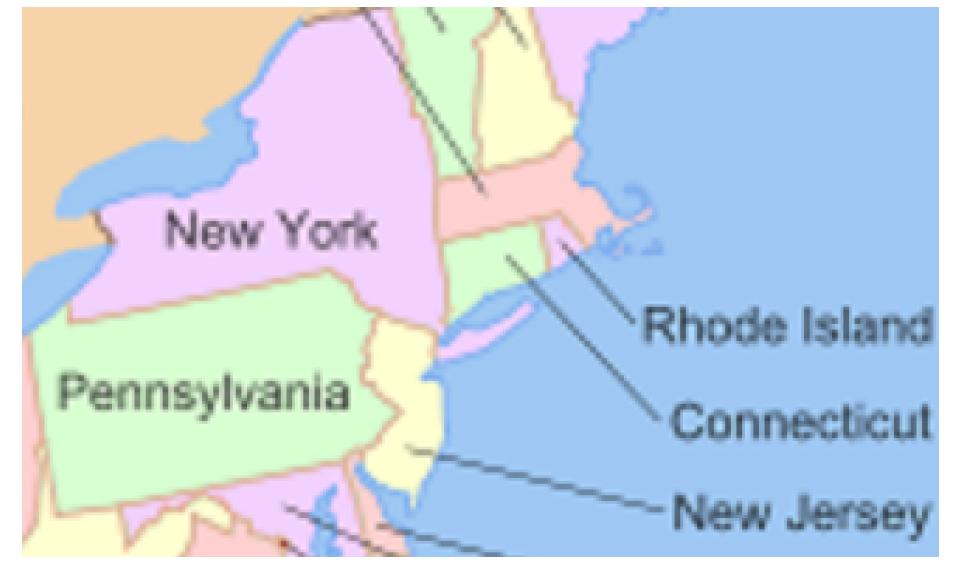
\includegraphics{figure/did-1.jpg}
\end{figure}
\end{center}
\item They surveyed about 400 fast food stores both in NJ and in PA both before and after the minimum wage increase in NJ.
\end{itemize}
\end{frame}





\begin{frame}{A Motivating Example}{Card \& Krueger (1994)}
\begin{itemize}
\item Two groups:
\vspace{0.2cm} 
\begin{itemize}
\item Treatment group: NJ
\vspace{0.2cm} 
\item Control group: PA
\end{itemize}
\vspace{0.2cm} 
\item Two periods:
\vspace{0.2cm} 
\begin{itemize}
\item Pre-treatment period: February 1992
\vspace{0.2cm} 
\item Post-treatment period: November 1992
\end{itemize}
\vspace{0.2cm} 
\item Let $Y_{st}$ denote the average employment in state $s$ at time $t$  	

\end{itemize}	
%	\begin{align*}
%	& Y_{ist}(1) \text{: employment at restaurant }i, \text{ state } s, \text{ time }t \text{ with a high } w^{\text{min}}\\
%	& Y_{ist}(0) \text{: employment at restaurant }i, \text{ state } s, \text{ time }t \text{ with a low } w^{\text{min}}
%	\end{align*}
%Potential outcomes:
%	\begin{itemize}
%	\item $Y_{iFeb}(1)$: outcome unit $i$ attains in period $t$ if treated before $t$
%	\item $Y_{0Feb}(t)$: outcome unit $i$ attains in period $t$ if not treated before $t$
%	\end{itemize}
\end{frame}





\begin{frame}{A Motivating Example}{Card \& Krueger (1994)}



\begin{itemize}
\item To estimate the effect of minimum wage on employment in NJ, we would like to know the following counterfactual:
\vspace{0.2cm}
\begin{itemize}
\item \textbf{In absence of raising minimum wage to \$5.05}, what the average employment level in NJ would be ?
\end{itemize}
\vspace{0.2cm}
\item DID design suggests us construct the \textbf{counterfactual employment in NJ} by using: 
\begin{itemize}
\item Average employment level in NJ before reform $+$
\vspace{0.2cm}
\item The trend in average employment level in PA (control group)
\end{itemize}
\vspace{0.2cm}
\begin{equation*}
Y_{NJ,Feb} + (Y_{PA,Nov} - Y_{PA,Feb})
\end{equation*}

\end{itemize}
\end{frame}




\begin{frame}{A Motivating Example}{Card \& Krueger (1994)}
\begin{itemize}
\item We can identify the effect of minimum wage on employment in NJ by taking difference in \textbf{realized employment} and \textbf{counterfactual employment} in NJ:
\begin{align*}
\alpha_{DID} &=  Y_{NJ,Nov} - {\color{red}[Y_{NJ,Feb} + (Y_{PA,Nov} - Y_{PA,Feb})]}  \\
&= (Y_{NJ,Nov} - Y_{NJ,Feb}) - (Y_{PA,Nov} - Y_{PA,Feb})
\end{align*}

\item If PA is a good control group:	
\vspace{0.2cm}
\begin{itemize}
\item The trend in employment rate of PA should absorb any other changes in employment that are unrelated to increase minimum wage	
\end{itemize}
\end{itemize}

\end{frame}


% \begin{frame}{A Motivating Example}{Card \& Krueger (1994)}
% \begin{figure}
% \tikzstyle{R} = [rectangle, text centered, draw = black]
% \begin{tikzpicture}[comment/.style={rectangle, text centered}]
% \centering
% \draw[black, thick] (0,0) -- (0,4) node[anchor=north west, yshift=3em, xshift=-5em] {Employment};
% \draw[black, thick] (2,0) -- (5,0) node[anchor=south east, yshift=-3em, xshift=4em] {Time};

% \foreach \x in {2}
% \draw (\x cm,1pt) -- (\x cm,-1pt) node[anchor=north] {$Feb$};
% \foreach \x in {5}
% \draw (\x cm,1pt) -- (\x cm,-1pt) node[anchor=north] {$Nov$};

% \foreach \y in {0}
% \draw (1pt,\y cm) -- (-1pt,\y cm) node[anchor=east] {$16$};
% \foreach \y in {1}
% \draw (1pt,\y cm) -- (-1pt,\y cm) node[anchor=east] {$18$};
% \foreach \y in {2}
% \draw (1pt,\y cm) -- (-1pt,\y cm) node[anchor=east] {$20$};
% \foreach \y in {3}
% \draw (1pt,\y cm) -- (-1pt,\y cm) node[anchor=east] {$22$};
% \foreach \y in {4}
% \draw (1pt,\y cm) -- (-1pt,\y cm) node[anchor=east] {$24$};

% \filldraw[black] (2,2) circle (1.5pt) node[anchor=west, xshift=-5em, yshift=1em] {\small Treated group (NJ)};
% \filldraw[black] (5,2) circle (1.5pt);
% \filldraw[black] (5,1) circle (1.5pt) node[anchor=west, yshift=-1em](ct) {\small Counterfacutal NJ};
% \node [comment, below of = ct, yshift=1.5em] {\small without treatment};

% \filldraw[black] (2,3.3) circle (1.5pt) node[anchor=west, xshift=-5em, yshift=1em] {\small Control group (PA)};
% \filldraw[black] (5,2.3) circle (1.5pt);

% \draw[black, thick] (2,2) -- (5,2);
% \draw[dashed, black, thick] (2,2) -- (5,1);
% \draw[black, thick] (2,3.3) -- (5,2.3);

% %\draw[dashed, gray] (0,0.5) -- (1,0.5);
% %\draw[dashed, gray] (0,2) -- (4,2);
% %\draw[dashed, gray] (0,2.5) -- (1,2.5);
% %\draw[dashed, gray] (0,5) -- (4,5);
% \end{tikzpicture}
% \end{figure}
% \end{frame}




\begin{frame}{A Motivating Example}{Card \& Krueger (1994)}
\begin{center}
\begin{threeparttable}
\centering\footnotesize
\begin{tabular}{clccc}
& & \multicolumn{3}{c}{Stores by state}\\
\cmidrule(l){3-5}
& &       &       & Difference, \\
& & PA    & NJ    & NJ-PA \\
\multicolumn{2}{l}{Variable} & (i)   & (ii)  & (iii) \\
\midrule
1.& Mean employment at         & 23.33  & 20.44  & -2.89 \\
&  February 1992             & (1.35) & (0.51) &(1.44) \\
2.& Mean employment at         & 21.17  & 21.03  & -0.14 \\
& November 1992              & (0.94) & (0.52) &(1.07) \\
3.& Change in mean employment  & -2.16  & 0.59   & \color{red}{2.76}   \\
& between Feb and Nov        & (1.25) & (0.54) & \color{red}{(1.44)} \\
\bottomrule
\end{tabular}
\end{threeparttable}
\end{center}
\begin{itemize}
\item Surprisingly, employment rose in NJ relative to PA after the minimum wage change.
\end{itemize}
\end{frame}



\begin{frame}{A Motivating Example}{Card \& Krueger (1994)}
	
	\begin{equation*}
		\begin{aligned}
			\alpha_{DID} &=  (Y_{NJ,Nov} - Y_{NJ,Feb}) {\color{red}- (Y_{PA,Nov} - Y_{PA,Feb})}  \\
			&=    (21.03 - 20.44) - (21.17 - 23.33)  \\
			&=  0.59 - (-2.16)  = 2.76
		\end{aligned}
	\end{equation*}
	\begin{itemize}
		\item Instead of comparing the employment of NJ in February (before reform) and November (after reform)
		\vspace{0.2cm}
		\item DID suggests we need to adjust for change (trend) in labor demand when there was no increase in minimum wage
		
	\end{itemize}
\end{frame}


\title[]  
{Identification}


\author 
{}

%\institute{Institute of Economics, Academia Sinica  \\ Econ, NTU}
%\institute{Institute of Economics, Academia Sinica  \\ IMES/IDAS, NCCU}
\institute{}

%\author 
%{楊子霆 \\ 中研院經濟所}

%\institute 
%{中正大學國際經濟專題研討}




\date
{}


\begin{frame}{}
	\titlepage
\end{frame}




\begin{frame}{Potential Outcomes Framework}{}
\begin{itemize}



\item Basic setup: two time periods, two groups
\vspace{0.2cm}
\item Two periods
\vspace{0.2cm}
\begin{itemize}
\item In period $t=1$: one of the groups is treated
\vspace{0.2cm}
\item In period $t=0$: neither group is treated
\vspace{0.2cm}
\end{itemize}
\item Two groups
\vspace{0.2cm}
\begin{itemize}
\item $D_i=1$: those that are treated at $t=1$ (treatment group)
\vspace{0.2cm}
\item $D_i=0$: those that are always untreated (control group)
\end{itemize}

\end{itemize}
\end{frame}




\begin{frame}{Potential Outcomes Framework}{}
\begin{itemize}
\item \textcolor{blue}{Potential Outcomes}
\vspace{0.2cm}
\begin{itemize}
\item $\mathrm{Y}^{1}_{it}$: the potential outcome for unit $i$ if he would receive treatment at time $t$
\vspace{0.2cm}
\item $\mathrm{Y}^{0}_{it}$: the potential outcome for unit $i$ if he would NOT receive treatment at time $t$
\end{itemize}

\end{itemize}
\end{frame}





\begin{frame}{Potential Outcomes Framework}{}
\begin{itemize}

\item \textcolor{blue}{Observed Outcomes}
\vspace{0.2cm}
\begin{itemize}
\item $Y_{it}$ is the observed outcome for unit $i$ at time $t$
\vspace{0.2cm}	


\begin{itemize}

\item Observed outcomes at $t=0$:
\begin{equation*}
Y_{i0}=\mathrm{Y}^{0}_{i0}
\end{equation*}
\item Observed outcomes at $t=1$: 
\begin{equation*}
Y_{i1}=\mathrm{Y}^{0}_{i1}(1-D_i)+\mathrm{Y}^{1}_{i1}D_i
\end{equation*}

\end{itemize}
%\item Treatment effect for unit $i$ at time $t=1$ is 
%	\begin{equation*}
%	\mathrm{Y}^{1}_{i1}-\mathrm{Y}^{0}_{i1}
%	\end{equation*}
\end{itemize}
\end{itemize}
\end{frame}


\begin{frame}{Identification Results for DID}
\begin{itemize} 
\item Our main interest is average treatment effect on treated (ATT):
\begin{equation*}
\alpha_{\text{ATT}}=E[\mathrm{Y}^{1}_{i1}-\mathrm{Y}^{0}_{i1}|D_{i}=1]
\end{equation*}
\vspace{0.2cm}
\item Missing data problem: $E[\mathrm{Y}^{0}_{i1}|D_{i}=1]$ is unknown
\vspace{0.3cm}
\item DID design can help us identify ATT if Parallel Trends Assumption holds

\end{itemize}
\end{frame}





\begin{frame}{Identification Results for DID}{Identification Assumption}
\begin{itemize} 

\begin{block}{Parallel Trends Assumption}
\begin{align*}
E[\mathrm{Y}^{0}_{i1}-\mathrm{Y}^{0}_{i0}|D_{i}=1]&=E[\mathrm{Y}^{0}_{i1}-\mathrm{Y}^{0}_{i0}|D_{i}=0]  \\
&=E[\mathrm{Y}_{i1}-\mathrm{Y}_{i0}|D_{i}=0]
\end{align*}
\end{block}
\item The treatment group and control group would have exhibited the same trend in the absence of the treatment
\vspace{0.2cm}
\item We can use Parallel Trends Assumption to construct a counterfactual for treatment group at $t=1$
\begin{align*}
\mathrm{E}[\mathrm{Y}^{0}_{i1} |D_{i}=1] &= \mathrm{E}[\mathrm{Y}^{0}_{i0}|D_{i}=1] + \mathrm{E}[\mathrm{Y}^{0}_{i1}-\mathrm{Y}^{0}_{i0}|D_{i}=0]  \\
&= \mathrm{E}[\mathrm{Y}_{i0}|D_{i}=1] + \mathrm{E}[\mathrm{Y}_{i1}-\mathrm{Y}_{i0}|D_{i}=0]
\end{align*}

\item We can use \textbf{observed outcomes} to represent \textbf{unobserved $\mathrm{E}[\mathrm{Y}^{0}_{i1} |D_{i}=1]$}

\end{itemize}
\end{frame}





\begin{frame}{Identification Results for DID}
\begin{itemize} 
\item Apply Parallel Trends Assumption:
\begin{align*}
\alpha_{\text{ATT}}&=\mathrm{E}[\mathrm{Y}^{1}_{i1}-\mathrm{Y}^{0}_{i1}|D_{i}=1] \\
&= \mathrm{E}[\mathrm{Y}^{1}_{i1}|D_{i}=1] - {\color{red}\mathrm{E}[\mathrm{Y}^{0}_{i1}|D_{i}=1]} \\
&= \mathrm{E}[\mathrm{Y}^{1}_{i1}|D_{i}=1] - {\color{red}\mathrm{E}[\mathrm{Y}^{0}_{i0}|D_{i}=1] - \mathrm{E}[\mathrm{Y}^{0}_{i1}-\mathrm{Y}^{0}_{i0}|D_{i}=0]} \\
&= \mathrm{E}[\mathrm{Y}^{1}_{i1}- \mathrm{Y}^{0}_{i0}|D_{i}=1] - \mathrm{E}[\mathrm{Y}^{0}_{i1}-\mathrm{Y}^{0}_{i0}|D_{i}=0]   \\
&= \mathrm{E}[\mathrm{Y}_{i1}- \mathrm{Y}_{i0}|D_{i}=1] - \mathrm{E}[\mathrm{Y}_{i1}-\mathrm{Y}_{i0}|D_{i}=0] = \alpha_{\text{DID}}
\end{align*}

\item The \textbf{average treatment effect on treated (ATT)} can be identified by difference in trend of outcome between treatment and control groups	

\end{itemize}
\end{frame}



\begin{frame}{Identification Results for DID}{Graphical Interpretation}
\begin{figure}
	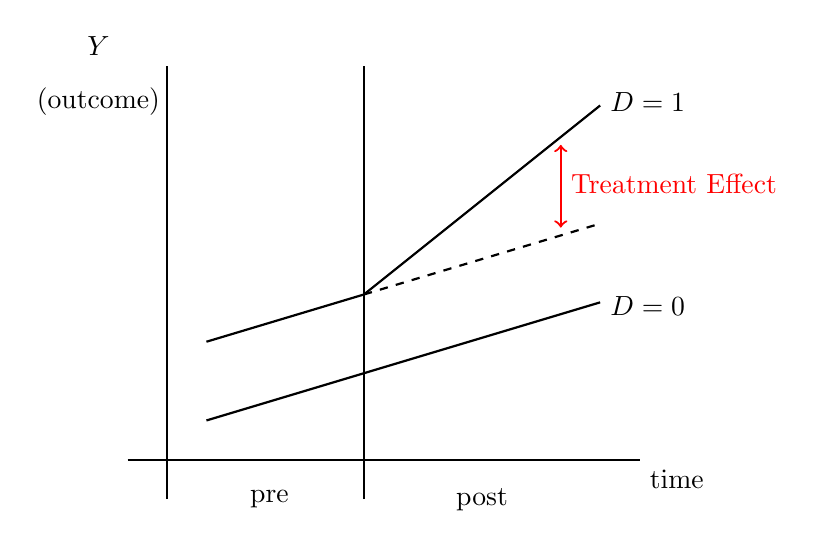
\begin{tikzpicture}[comment/.style={rectangle, text centered}]
	\centering
	\draw [thick] (-0.5,0) -- (6,0) node[anchor=north west] {time};
	\draw [thick] (0,-0.5) -- (0,5) node[anchor=south east, xshift=-0.6cm](Y) {$Y$};
	\node [comment, below of = Y, yshift=0.3cm] {(outcome)};
	
	\draw [thick] (2.5,-0.5) -- (2.5,5);
	
	\draw [thick] (0.5,0.5) -- (5.5,2) node[anchor=north west, yshift=0.2cm] {$D=0$};
	\draw [thick] (0.5,1.5) -- (2.5,2.1);
	\draw [thick] (2.5,2.1) -- (5.5,4.5) node[anchor=north west, yshift=0.3cm] {$D=1$};
	\draw [thick,dashed] (2.5,2.1) -- (5.5,3);
	
	\draw [thick,<->, red] (5,2.95) -- (5,4) node[anchor=west, yshift=-0.5cm] {Treatment Effect};
	
	\draw (1.3,0)--(1.3,0) node (1.3_0) {};
	\node [comment, below of = 1.3_0, yshift=0.5cm] {pre};
	
	\draw (4,0)--(4,0) node (4_0) {};
	\node [comment, below of = 4_0, yshift=0.5cm] {post};
	
	\end{tikzpicture}
\end{figure}
\end{frame}




\title[]  
{Estimation}


\author 
{}

%\institute{Institute of Economics, Academia Sinica  \\ Econ, NTU}
%\institute{Institute of Economics, Academia Sinica  \\ IMES/IDAS, NCCU}
\institute{}

%\author 
%{楊子霆 \\ 中研院經濟所}

%\institute 
%{中正大學國際經濟專題研討}




\date
{}


\begin{frame}{}
	\titlepage
\end{frame}



%-------------------------------------------------------
% Frame 1: DID Estimation — Basic Setup
%-------------------------------------------------------
\begin{frame}{DID Estimation}{Basic Two-Period/Two-Group Setup}
\begin{itemize}
    \item Basic case: two groups (treatment \& control) and two periods (pre \& post)
    \vspace{0.2cm}
    \item We implement the DID design using a simple regression:
    \begin{equation*}
        Y_{it} = \mu + \gamma D_{i} + \delta Post_{t} + \alpha (D_{i} \times Post_{t}) + \varepsilon_{it}
    \end{equation*}
    \item Each coefficient has a clear economic interpretation:
    \vspace{0.2cm}
    \begin{itemize}
        \item $D_i = 1$: individual $i$ belongs to the \textbf{treatment group}
        \vspace{0.2cm}
        \item $Post_t = 1$: period $t$ is the \textbf{post-treatment period}
        \vspace{0.2cm}
        \item $\gamma$: time-invariant difference between treatment and control group
        \vspace{0.2cm}
        \item $\delta$: time trend common to all groups (regardless of treatment)
        \vspace{0.2cm}
        \item $\alpha$: \textbf{treatment effect} --- the extra change in the treatment group \emph{beyond} the common trend
    \end{itemize}
\end{itemize}
\end{frame}




%-------------------------------------------------------
% Frame 2: DID as a Difference in Means
%-------------------------------------------------------
\begin{frame}{DID Estimation}{$\alpha$ as the DID Estimator}

\begin{equation*}
    Y_{it} = \mu + \gamma D_{i} + \delta Post_{t} + \alpha (D_{i} \times Post_{t}) + \varepsilon_{it}
\end{equation*}

\begin{itemize}
    \item The coefficient $\alpha$ on the interaction term $D_i \times Post_t$ captures:
            \vspace{0.2cm}

    \begin{itemize}
        \item The differential trend in outcomes between the treatment and control groups after treatment happened
        %\item i.e., how much \emph{more} the treatment group changed relative to the control group
    \end{itemize}
    \vspace{0.2cm}
    \item We will show that $\alpha$ equals the standard DID formula:
    \begin{align*}
        \alpha_{DID} &= \underbrace{\bigl[\mathrm{E}[Y_{it}|D_i=1, Post_t=1] - \mathrm{E}[Y_{it}|D_i=1, Post_t=0]\bigr]}_{\text{change in treatment group}} \\[4pt]
        &\quad - \underbrace{\bigl[\mathrm{E}[Y_{it}|D_i=0, Post_t=1] - \mathrm{E}[Y_{it}|D_i=0, Post_t=0]\bigr]}_{\text{change in control group (common trend)}}
    \end{align*}
\end{itemize}
\end{frame}


\begin{frame}{DID Estimation}{Proof: $\alpha = \alpha_{DID}$}

\begin{align*}
    \alpha_{DID}
    &= \underbrace{\bigl[\mathrm{E}[Y_{it}|D_i=1, Post_t=1] - \mathrm{E}[Y_{it}|D_i=1, Post_t=0]\bigr]}_{\text{change in treatment group}}  \\[4pt]
    &\quad - \underbrace{\bigl[\mathrm{E}[Y_{it}|D_i=0, Post_t=1] - \mathrm{E}[Y_{it}|D_i=0, Post_t=0]\bigr]}_{\text{change in control group (common trend)}} \\[8pt]
    &= \bigl[(\mu+\gamma+\delta+\alpha) - (\mu+\gamma)\bigr]
     - \bigl[(\mu+\delta) - \mu\bigr] \\[4pt]
    &= (\delta + \alpha) - \delta \\[4pt]
    &= \alpha
\end{align*}

\begin{itemize}
    \item  Under $E[\varepsilon_{it} \mid D_i, Post_t] = 0$, the OLS coefficient $\alpha$ on $D_i \times Post_t$ \textbf{equals the DID treatment effect} $\alpha_{DID}$.
\end{itemize}

% \begin{alertblock}{Key Result}
%     Under $E[\varepsilon_{it} \mid D_i, Post_t] = 0$, the OLS coefficient $\alpha$ on $D_i \times Post_t$ \textbf{equals the DID treatment effect} $\alpha_{DID}$.
% \end{alertblock}

\end{frame}







% %-------------------------------------------------------
% % Frame 3: Conditional Means Table
% %-------------------------------------------------------
% \begin{frame}{DID Estimation}{Computing Conditional Means}

% \begin{equation*}
%     Y_{it} = \mu + \gamma D_{i} + \delta Post_{t} + \alpha (D_{i} \times Post_{t}) + \varepsilon_{it}
% \end{equation*}

% \begin{itemize}
%     \item Assume $E[\varepsilon_{it} \mid D_i, Post_t] = 0$ (no omitted confounders conditional on group and period)
%     \vspace{0.3cm}
%     \item The four group-period conditional means are:
% \end{itemize}

% \vspace{0.2cm}
% \begin{center}
% \begin{threeparttable}
% \begin{tabular}{lcc}
% \toprule
%                   & Pre ($Post=0$)       & Post ($Post=1$)                  \\
% \midrule
% Control ($D=0$)   & $\mu$                & $\mu + \delta$                   \\[4pt]
% Treatment ($D=1$) & $\mu + \gamma$       & $\mu + \gamma + \delta + \alpha$ \\
% \bottomrule
% \end{tabular}
% \begin{tablenotes}
% \small
% \item $\gamma$ = level difference between groups; $\delta$ = common time trend; $\alpha$ = treatment effect
% \end{tablenotes}
% \end{threeparttable}
% \end{center}

% \end{frame}


% %-------------------------------------------------------
% % Frame 4: Deriving alpha = alpha_DID
% %-------------------------------------------------------
% \begin{frame}{DID Estimation}{Proof: $\alpha = \alpha_{DID}$}

% \begin{itemize}
%     \item Using the conditional means from the table, the DID formula gives:
%     \begin{align*}
%         \alpha_{DID}
%         &= \bigl[(\mu+\gamma+\delta+\alpha) - (\mu+\gamma)\bigr]
%          - \bigl[(\mu+\delta) - \mu\bigr] \\[4pt]
%         &= (\delta + \alpha) - \delta \\[4pt]
%         &= \alpha
%     \end{align*}

%     \vspace{0.2cm}
%     \item Intuition: by subtracting the control group's change ($\delta$), we \textbf{remove the common time trend} and isolate the causal effect
% \end{itemize}

% \begin{alertblock}{Key Result}
%     Under $E[\varepsilon_{it} \mid D_i, Post_t] = 0$, the OLS coefficient $\alpha$ on $D_i \times Post_t$ \textbf{equals the DID treatment effect} $\alpha_{DID}$.
% \end{alertblock}

% \end{frame}


%-------------------------------------------------------
% Frame 5: Summary Table
%-------------------------------------------------------
\begin{frame}{DID Estimation}{Summary: Decomposing the DID Estimator}

\begin{center}
\begin{threeparttable}
\begin{tabular}{lccc}
\toprule
                     & Pre                 & Post                             & $\Delta$ (Post $-$ Pre) \\
\midrule
Control ($D=0$)      & $\mu$               & $\mu + \delta$                   & $\delta$                \\[4pt]
Treatment ($D=1$)    & $\mu + \gamma$      & $\mu + \gamma + \delta + \alpha$ & $\delta + \alpha$       \\[4pt]
\midrule
\textbf{DID}         &                     &                                  & $\boldsymbol{\alpha}$   \\
\bottomrule
\end{tabular}
% \begin{tablenotes}
% \small
% \item The DID estimator differences out $\delta$ (common trend), leaving only $\alpha$ (treatment effect).
% \end{tablenotes}
\end{threeparttable}
\end{center}

\begin{itemize}
    \item Both groups share the same time trend $\delta$:  This is the \textbf{parallel trends assumption}
    \vspace{0.2cm}
    \item By differencing, we remove $\delta$ and recover the causal effect $\alpha$
\end{itemize}

\end{frame}







% \begin{frame}{DID Estimation}{Basic Two Periods/Groups}
% \begin{itemize}
% \item Basic case: two groups and two periods
% \vspace{0.2cm}
% \item We can obtain the DID estimates using a regression framework
% \vspace{0.2cm}	
% %\item To implement DID method in a regression framework, we estimate:
% \begin{equation*}
% Y_{it}=\mu+\gamma D_{i} + \delta Post_{t} + \alpha (D_{i} \times Post_{t})+\varepsilon_{it},
% \end{equation*}

% \begin{itemize}
% \item $D$ is a dummy indicating treatment group
% \vspace{0.2cm}
% \item $Post$ is a dummy indicating post-treatment period
% \vspace{0.2cm}
% %\item $\varepsilon_{st}$ is a transitory shock/idiosyncratic error
% %\vspace{0.2cm}
% \item $\gamma$ captures differences across groups that are constant over time
% \vspace{0.2cm}
% \item $\delta$ captures differences over time that are common to all groups
% \vspace{0.2cm}


% %\item if $E[\varepsilon|D,T]=0$
% \end{itemize}

% \end{itemize}
% \end{frame}



% \begin{frame}{DID Estimation}{Basic Two Periods/Groups}
	
% 	\begin{equation*}
% Y_{it}=\mu+\gamma D_{i} + \delta Post_{t} + \alpha (D_{i} \times Post_{t})+\varepsilon_{it},
% 	\end{equation*}
	
% 	\begin{itemize}
% 	\item $\alpha$ is the coefficient of interest 
% 	\vspace{0.2cm}
% 	\begin{itemize}
% 		\item Capture the different trends in outcome between treatment and control group
% 	\end{itemize}
	
% \item We will show that $\alpha$ can represent the DID estimate:
% \begin{align*}
% 		\alpha &= \{\mathrm{E}[\mathrm{Y}_{it}|D_{i}=1,Post_{t}=1]-\mathrm{E}[\mathrm{Y}_{it}|D_{i}=1,Post_{t}=0]\} \\
% 		&- \{\mathrm{E}[\mathrm{Y}_{it}|D_{i}=0,Post_{t}=1]-\mathrm{E}[\mathrm{Y}_{it}|D_{i}=0,Post_{t}=0]\}
% 		%&= \{(\mu + \gamma + \delta + \alpha_{DID}) - (\mu + \gamma)\} - \{(\mu + \delta) - \mu\}
% \end{align*}	
	
	
	
% 		\end{itemize}
		
		

% \end{frame}





% \begin{frame}{DID Estimation}{Basic Two Periods/Groups}

% \begin{equation*}
% Y_{it}=\mu+\gamma D_{i} + \delta Post_{t} + \alpha (D_{i} \times Post_{t})+\varepsilon_{it},
% \end{equation*}

% \begin{itemize}
% \item Assume $E[\varepsilon_{it}|D,Post]=0$
% \vspace{0.2cm}
% %\iten Then, we can show that
% \begin{itemize}
% \item \textbf{Pre-treatment mean of outcome for control group:} $\mathrm{E}[\mathrm{Y}_{it}|D=0,Post=0]=\mu$
% \vspace{0.2cm}
% \item \textbf{Post-treatment mean of outcome for control group:} $\mathrm{E}[\mathrm{Y}_{it}|D=0,Post=1]=\mu + \delta$
% \vspace{0.2cm}
% \item \textbf{Pre-treatment mean of outcome for treatment group:} $\mathrm{E}[\mathrm{Y}_{it}|D=1,Post=0]=\mu + \gamma$ 
% \vspace{0.2cm}
% \item \textbf{Post-treatment mean of outcome for treatment group:} $\mathrm{E}[\mathrm{Y}_{it}|D=1,Post=1]=\mu + \gamma + \delta + \alpha$
% \vspace{0.2cm}
% \end{itemize}


% \end{itemize}
% \end{frame}



% \begin{frame}{DID Estimation}{Basic Two Periods/Groups}
% 	\begin{itemize}
		
% 		\item $\alpha$ can represent treatment effect identified by DID design $\alpha_{DID}$:
% 		\begin{align*}
% 				\alpha_{DID} &= \{\mathrm{E}[\mathrm{Y}_{it}|D=1,Post=1]-\mathrm{E}[\mathrm{Y}_{it}|D=1,Post=0]\} \\
% 				&- \{\mathrm{E}[\mathrm{Y}_{it}|D=0,Post=1]-\mathrm{E}[\mathrm{Y}_{it}|D=0,Post=0]\}  \\
% 				&= \{(\mu + \gamma + \delta + \alpha) - (\mu + \gamma)\} - \{(\mu + \delta) - \mu\} \\
% 				&= \alpha
% 		\end{align*}
		
% 	\end{itemize}
% \end{frame}



% \begin{frame}{DID Estimation}{Basic Two Periods/Groups}

% \begin{center}
% \begin{threeparttable}
% %\tabcolsep=0.9pt
% %\fontsize{9}{9pt}\selectfont
% \centering %\footnotesize
% %\caption{}
% %\extrarowheight = 4pt 
% \begin{tabular}{lccc}
% \toprule
% & Pre       & Post     & Pre/Post difference \\
% \midrule                                                                             
% Control Group    & $\mu$  & $\mu + \delta$ &  $\delta$ \\
% Treatment Group	    & $\mu + \gamma$  & $\mu + \gamma + \delta + \alpha$ & $ \delta + \alpha$ \\
% DID 	&              &          & $ \alpha$ \\
% \bottomrule
% \end{tabular}
% \end{threeparttable}
% \end{center}

% \end{frame}




%-------------------------------------------------------
% Frame 1: Advantages + Treatment Intensity (with D and Post)
%-------------------------------------------------------
\begin{frame}{DID Estimation}{Advantages of the Regression Framework}
\begin{itemize}
    \item Estimating the DID estimator in a regression framework has the following advantages: 
    \vspace{0.2cm}
    \begin{itemize}
        \item It is easy to calculate standard errors
        \vspace{0.2cm}
        \item We can control for other covariates $X_{it}$ to further reduce residual bias
        \vspace{0.2cm}
        \item It is easy to accommodate \textbf{multiple periods}
        \vspace{0.2cm}
        \item $D_i$ can be a \textbf{continuous} measure of treatment intensity
        \vspace{0.2cm}
        \begin{itemize}	
            \item Example: varying increases in the minimum wage across states
            \vspace{0.2cm}
            \item Estimating equation:
            \[
                Y_{it} = \mu + \gamma D_{i} + \delta Post_t + \alpha (D_{i} \times Post_t) + \varepsilon_{it}
            \]
            \item $\alpha$ captures the effect of a \textbf{one-unit increase} in treatment intensity
        \end{itemize}
    \end{itemize}
\end{itemize}
\end{frame}


%-------------------------------------------------------
% Frame 2: General DID with Two-Way FE
%-------------------------------------------------------
\begin{frame}{DID Estimation}{Generalization: Two-Way Fixed Effects}
\begin{itemize}
    \item The basic two-period setup can be generalized to \textbf{multiple periods and multiple groups}
    \vspace{0.2cm}
    \item Replace the group dummy $\gamma D_i$ and period dummy $\delta Post_t$ with \textbf{fixed effects}:
    \[
        Y_{it} = \alpha D_{it} + \lambda_i + \gamma_t + \varepsilon_{it}
    \]
    \vspace{0.1cm}
    \begin{itemize}
        \item $\lambda_i$: \textbf{unit fixed effects} --- absorb all time-invariant differences across units
        \vspace{0.2cm}
        \item $\gamma_t$: \textbf{time fixed effects} --- absorb common shocks across all units
        \vspace{0.2cm}
        \item $D_{it}$: treatment that can now vary across \emph{both} units and time
    \end{itemize}
    \vspace{0.2cm}
    \item This is called the \textbf{Two-Way Fixed Effects (TWFE)} estimator
\end{itemize}

% \begin{alertblock}{Parallel Trends in TWFE}
%     After controlling for unit and time FE, the identifying assumption is that \textbf{trends in outcomes would have been the same} across treated and untreated units in the absence of treatment.
% \end{alertblock}

\end{frame}





\title[]  
{Examine Parallel Trends Assumption}


\author 
{}

%\institute{Institute of Economics, Academia Sinica  \\ Econ, NTU}
%\institute{Institute of Economics, Academia Sinica  \\ IMES/IDAS, NCCU}
\institute{}

%\author 
%{楊子霆 \\ 中研院經濟所}

%\institute 
%{中正大學國際經濟專題研討}




\date
{}


\begin{frame}{}
	\titlepage
\end{frame}





\begin{frame}{Testing the Parallel Trends Assumption}{}
	\begin{itemize}
		\item The key assumption for any DID design is the \textbf{Parallel Trends Assumption}
		\vspace{0.2cm}
		\item The outcome in treatment and control groups would follow \textbf{the same time trend in the absence of the treatment}.
		\vspace{0.2cm}
		\begin{itemize}
			\item This does not mean that they have to have the same level (mean) of the outcome!
			\vspace{0.2cm}
			\item Parallel Trends Assumption is fundamentally untestable in the post-treatment period.
			\vspace{0.2cm}
			\item However, we can use \textbf{pre-treatment data} to provide supporting evidence for this assumption:
			\vspace{0.2cm}
			\begin{itemize}
				\item Graphical evidence showing similar pre-treatment trends
				\vspace{0.2cm}
				\item Formal tests using event study/dynamic DID specifications
								\vspace{0.2cm}
			\end{itemize}
			\item Even if pre-trends are similar, we should still be concerned about \textbf{other policies or events changing at the same time}
		\end{itemize}
	\end{itemize}
\end{frame}



\begin{frame}{Examining Parallel Pre-Trends}{Graphical Evidence}
	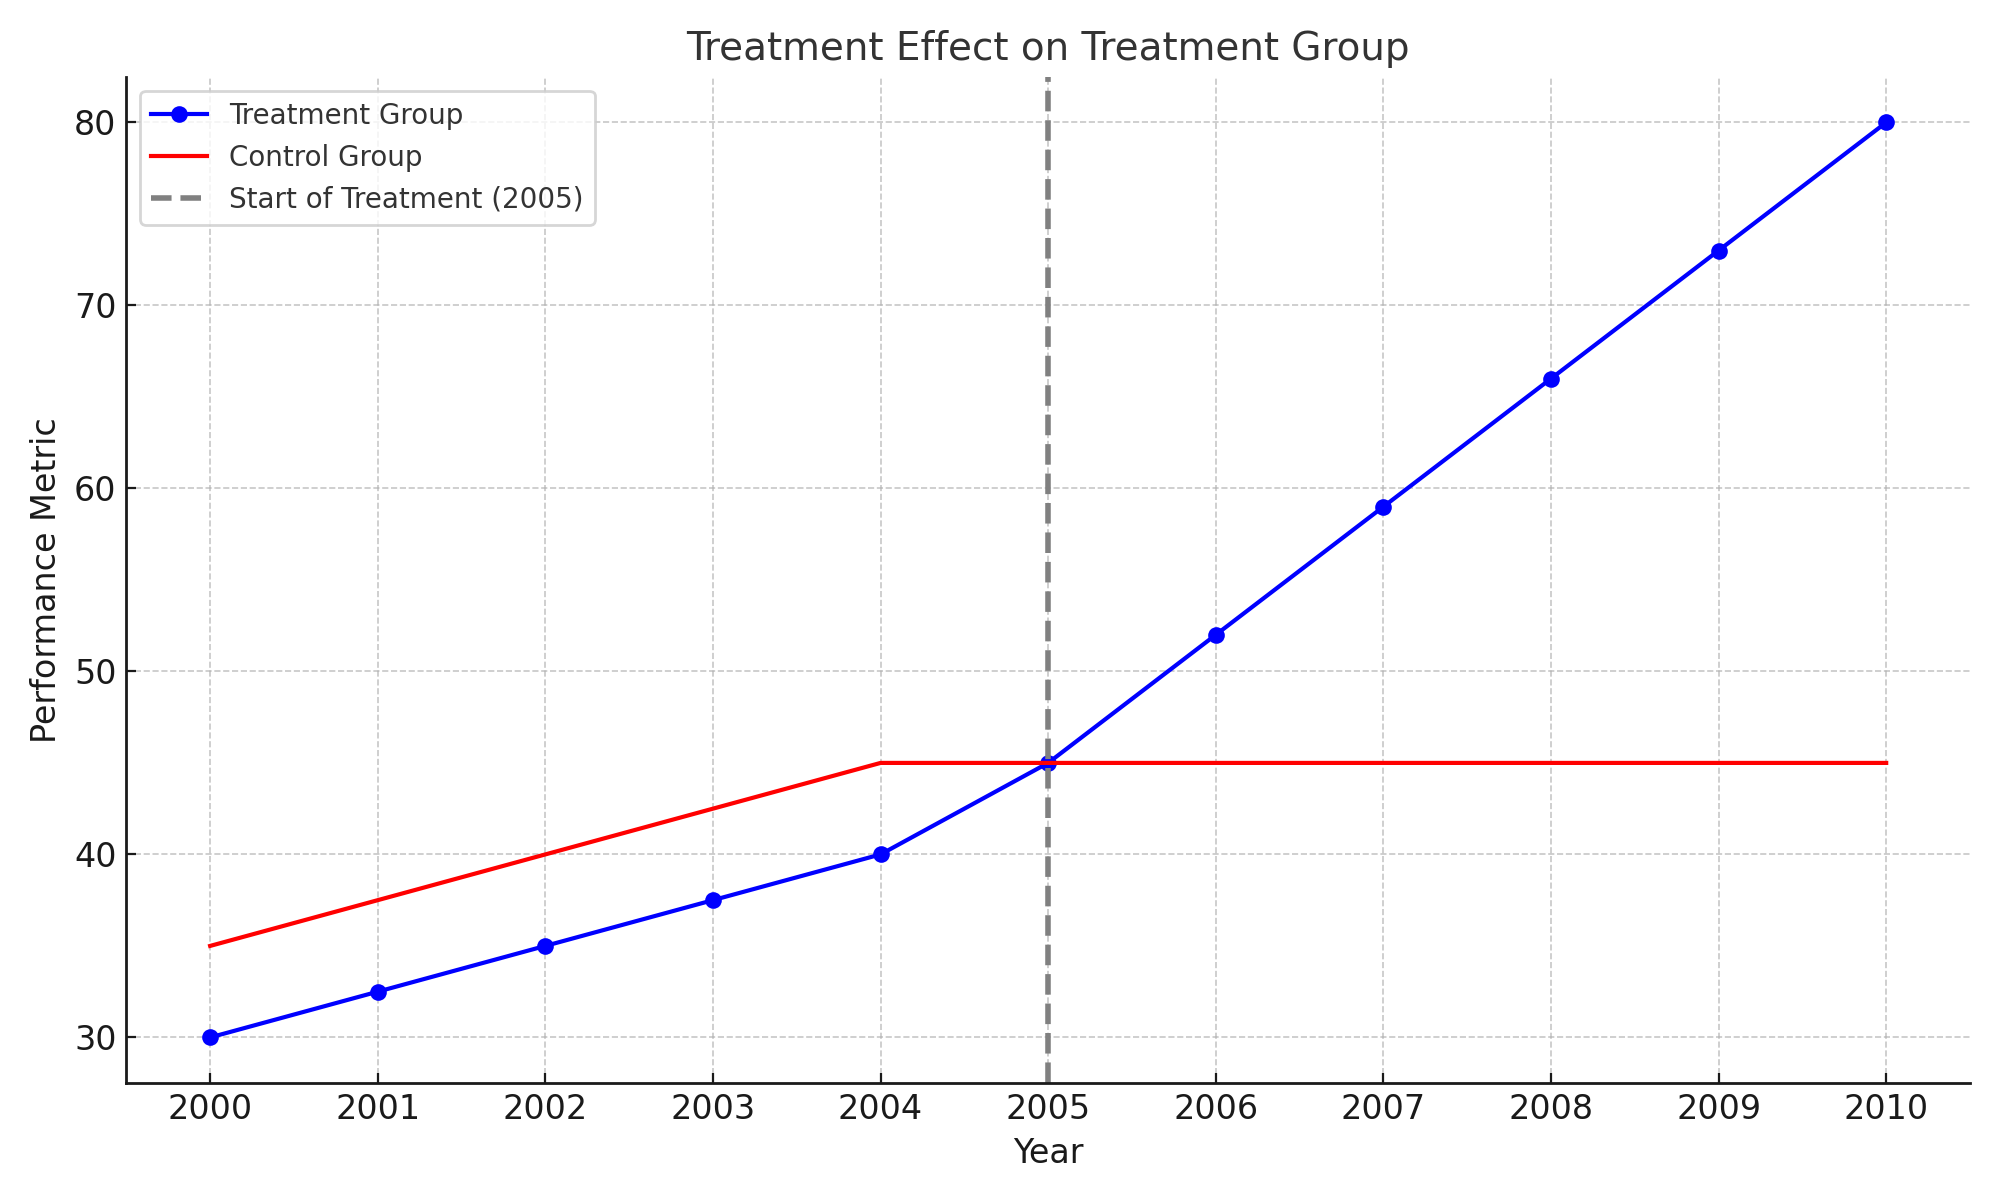
\includegraphics[width=1.0\textwidth]{figure/treatment_effect_minimal_change.png} 
	%\begin{itemize}
	%\hyperlink{sub_2}{\beamergotobutton{back}} 
	%\end{itemize}
\end{frame}



\begin{frame}{Examining Parallel Pre-Trends}{Graphical Evidence}
	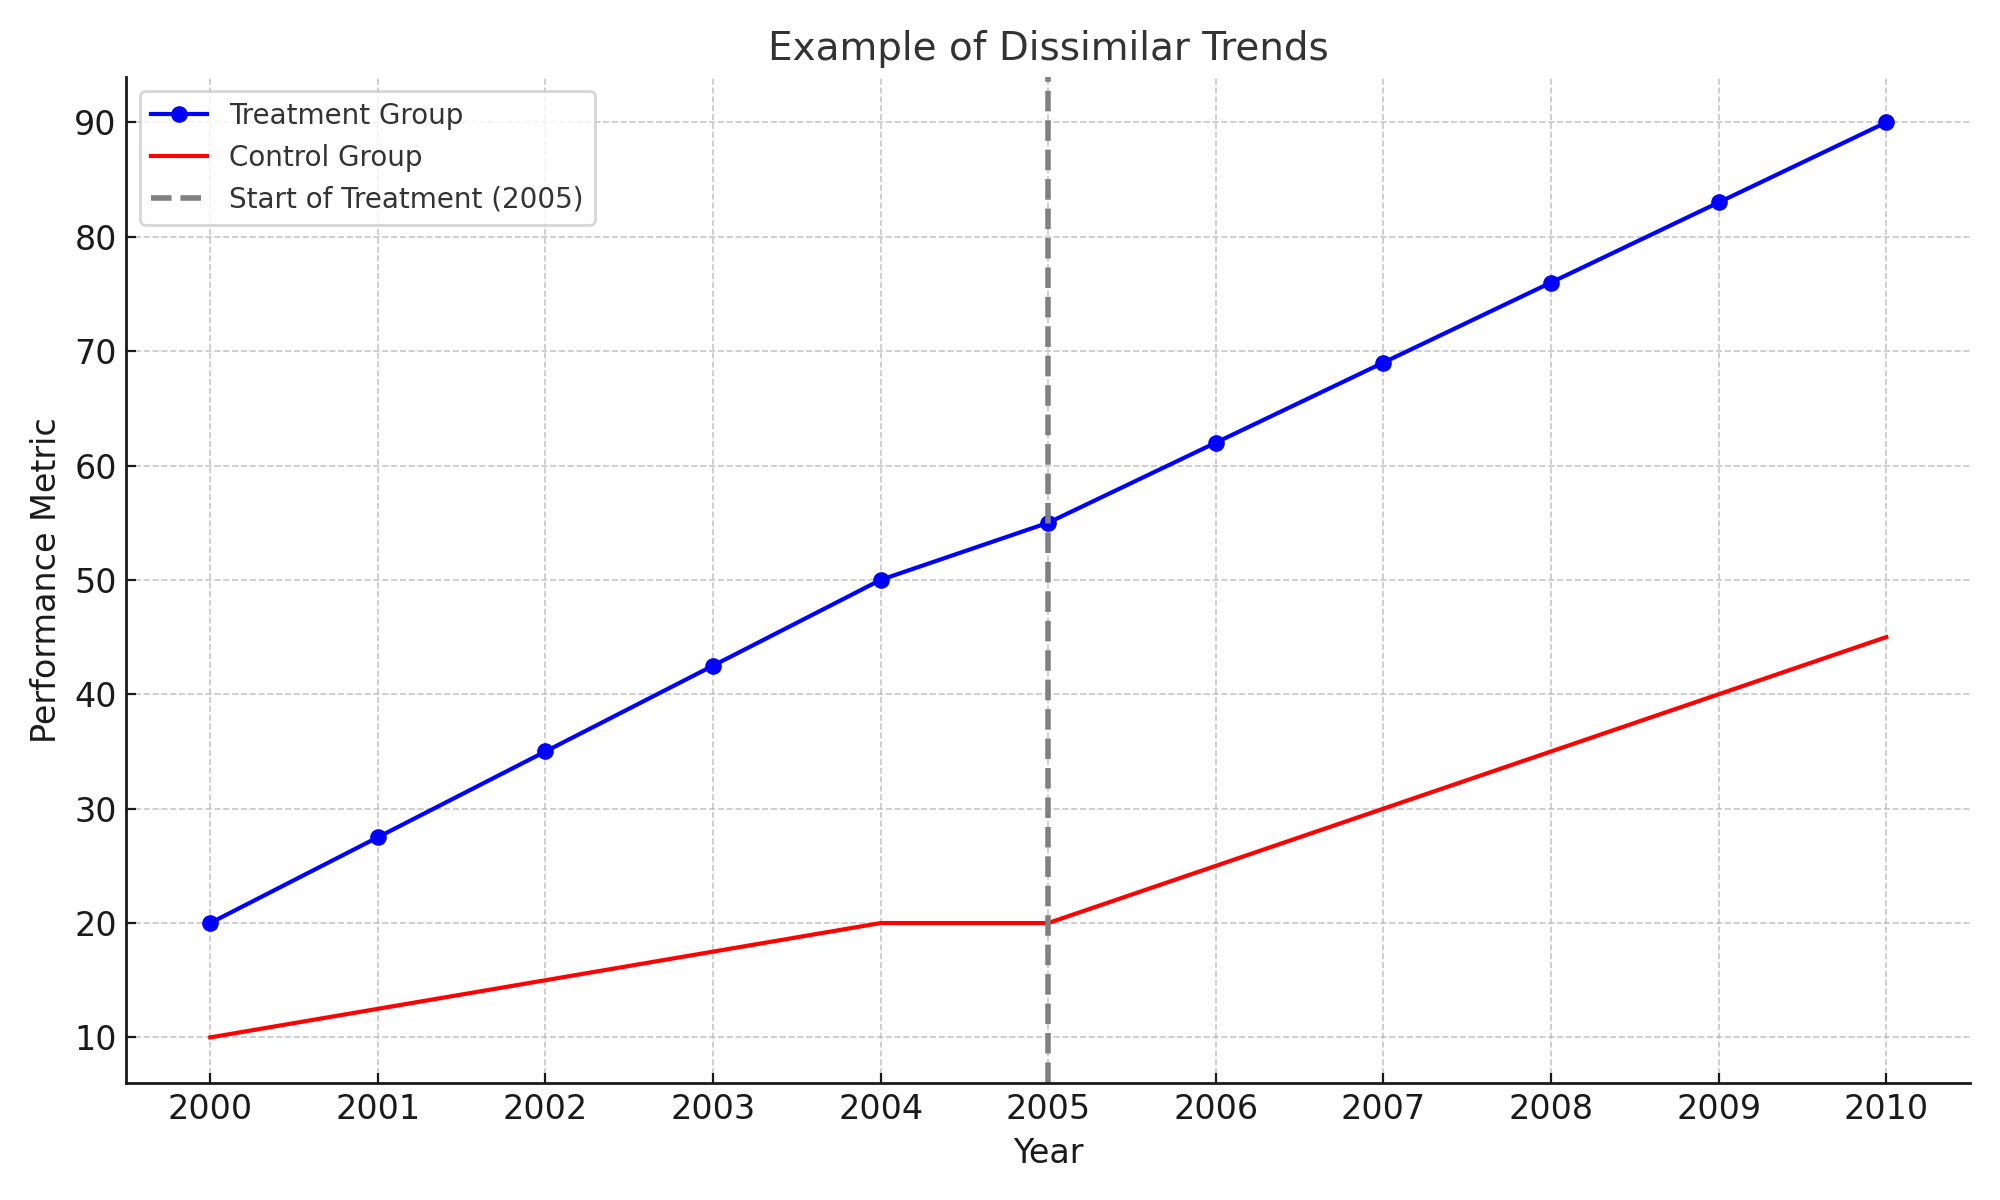
\includegraphics[width=1.0\textwidth]{figure/dissimilar_trend_english.png} 
	%\begin{itemize}
	%\hyperlink{sub_2}{\beamergotobutton{back}} 
	%\end{itemize}
\end{frame}





\begin{frame}{Dynamic DID Design}
	\begin{itemize}
		\item We can include leads and lags in the DID specification:
		\vspace{0.2cm}
		\begin{itemize}
			\item[1] To examine whether treatment and control group share similar pre-treatment trends
			\vspace{0.2cm}
			\item[2] To analyze whether the treatment effect changes over time after implementation 
		\end{itemize}
		\vspace{0.2cm}
		\item This approach is called the \textbf{Dynamic DID Design} or \textbf{Event-Study Design}
	
	
	\end{itemize}
\end{frame}



\begin{frame}{Dynamic DID Design}
	\begin{itemize}
		\item The estimated regression would be:
		\begin{align*}
		Y_{it}&=\alpha + \beta D_{i} + \sum^{q}_{\substack{k=-m\\k\neq-1}}\delta_{k} \mathbf{I}[t-E_{i}=k]  \\
		&+ \sum^{q}_{\substack{k=-m\\k\neq-1}}\gamma_{k} D_{i} \times \mathbf{I}[t-E_{i}=k]
		+X'_{it}\theta+\varepsilon_{it},
		\end{align*}
		\begin{itemize}
			%\vspace{0.3cm}
			\item  $E_{i}$ represents the timing when treatment happens.
			\vspace{0.2cm}
			\item $\mathbf{I}[t-E_{i}=k]$ is an indicator for being $k$ years from the treatment event
						\vspace{0.2cm}
			\item $t$ is the calendar year
						\vspace{0.2cm}
				\begin{itemize}			
			\item Treatment occurs in $k=0$ ($t=E_{i}$)
			\vspace{0.2cm}
			\item For example, $\mathbf{I}[t-E_{i}=-1]$ is a dummy variable indicating one year before treatment occurs
					\vspace{0.2cm}
			\item We usually use time $k=-1$ as baseline year
			
					\end{itemize}
					
		\end{itemize}
	\end{itemize}
\end{frame}





\begin{frame}{Dynamic DID Design}
	\begin{itemize}
		\item The estimated regression would be:
		\begin{align*}
				Y_{it}&=\alpha + \beta D_{i} + \sum^{q}_{\substack{k=-m\\k\neq-1}}\delta_{k} \mathbf{I}[t-E_{i}=k]  \\
				&+ \sum^{q}_{\substack{k=-m\\k\neq-1}}\gamma_{k} D_{i} \times \mathbf{I}[t-E_{i}=k]
				+X'_{it}\theta+\varepsilon_{it},
		\end{align*}
		\begin{itemize}
			\vspace{0.2cm}
			\item $\gamma_{-2}, \gamma_{-3},...,\gamma_{-m} $ represent pre-trend
			\vspace{0.2cm}
			\begin{itemize}			
				\item These coefficients should be zero if  pre-tends is parallel
				\vspace{0.2cm}
			\end{itemize}
			\item $\gamma_{0}, \gamma_{1},...,\gamma_{q} $ represent post-treatment effects
		\end{itemize}
	\end{itemize}
\end{frame}




\begin{frame}{Dynamic DID Design}{Example}
	
	
	Hsing-Wen Han, Kuang-Ta Lo, Yung-Yu Tsai, and Tzu-Ting Yang (2026), ``\textbf{The Effect of Financial Resources on Fertility: Evidence from Administrative Data on Lottery Winners}", \textit{Journal of Labor Economics}
	
	
	%\begin{itemize}
	%	\item Autor (2003) includes both leads and lags in a DID model analyzing the effect of increased employment protection on the firm's use of temporary help workers
	%\end{itemize}
	
\end{frame}


\begin{frame}{Empirical Example: Han et al. (2026)}{Motivation}
	\begin{itemize} 
		
			\item During the past fifty years, fertility rates in developed countries have declined dramatically
		\vspace{0.3cm}
		\item Low fertility rate leads to the growth of an aging population, workforce shortages, and reductions in tax revenue.
		\vspace{0.3cm}
		\item Many countries initiated child-related cash transfer policies to encourage childbearing.
		\vspace{0.3cm}
		\begin{itemize}
			\item On average, the public spending of child-related cash benefits accounts for 1.1\% of GDP in OECD countries.
			\vspace{0.3cm}
		\end{itemize}
		\item The rationale behind these policies is that people do not have enough income to afford the expense of raising children, so the government needs to subsidize them.
		
	\end{itemize}	
\end{frame}



\begin{frame}{Empirical Example: Han et al. (2026)}{Motivation}
	\begin{itemize} 
		
	\item Empirically, there is an endogenous problem between income and fertility.
	\vspace{0.3cm}
	\begin{itemize} 
		\item Reverse Causality
		\vspace{0.3cm}
		\item Income effect confounds with substitution effect
		\vspace{0.3cm}
		\begin{itemize} 
			
			\item Both working and raising children are time-consuming activities				
			\vspace{0.3cm}	
			
			\item A sudden increase in wage income can increase the relative price of having children
			\vspace{0.3cm}
			\item Higher wage income would make people work more and reduce demand for children
			
			
			%Income and fertility could be jointly determined
			\vspace{0.3cm}
		\end{itemize}
		\end{itemize}	
	\end{itemize}	
\end{frame}










\begin{frame}{Empirical Example: Han et al. (2026)}{Dynamic DID Design}
	\begin{itemize} 
			
		\item This paper examines the fertility
		impact of the large and permanent income shock generated by winning lottery prizes.
		\vspace{0.3cm}
		\item We implement a dynamic DID design to examine the causal effect of large income shock on fertility.
				\vspace{0.3cm}
		\item Compare the trend in fertility before and after receiving a windfall gain between:
						\vspace{0.3cm}
			\begin{itemize} 
		\item Households winning 1,000,000 NT\$ from lottery prizes.
								\vspace{0.3cm}
		\item Households winning less than 10,000 NT\$. 
			\end{itemize}	
		
	\end{itemize}	
\end{frame}




\begin{frame}{Empirical Example: Han et al. (2026)}{Dynamic DID Design}
	\begin{itemize} 
		\item We estimate the following regression:
		\begin{align*}
			Y_{it}&=\alpha + \beta D_{i} + \sum^{6}_{k=-3}\delta_{k} \mathbf{I}[t-E_{i}=k]  \\
			&+ \sum^{6}_{k=-3}\gamma_{k} D_{i} \times \mathbf{I}[t-E_{i}=k]
			+X'_{it}\theta+\varepsilon_{it},
		\end{align*}
	\begin{itemize} 
		\item $D_{i}$ represents treatment group dummy.	
						\vspace{0.3cm}
				\item Treatment Group:
			\vspace{0.3cm}
			\begin{itemize} 
				\item Households who earn more than 1,000,000 NT\$ by winning lotteries in a given year
			\end{itemize}
			\vspace{0.3cm}
			\item Control group:
			\vspace{0.3cm}
			\begin{itemize} 
				\item Households who earn less than 10,000 NT\$ from winning lotteries during sample period
			\end{itemize}		
				\end{itemize}
	\end{itemize}
\end{frame}











\begin{frame}{Empirical Example: Han et al. (2026)}{Dynamic DID Design}

	%	\item We estimate the following regression:
		\begin{equation*}
	\begin{aligned}
		Y_{it}&=\alpha + \beta D_{i} + \sum^{6}_{k=-3}\delta_{k} \mathbf{I}[t-E_{i}=k]  \\
		&+ \sum^{6}_{k=-3}\gamma_{k} D_{i} \times \mathbf{I}[t-E_{i}=k]
		+X'_{it}\theta+\varepsilon_{it},
	\end{aligned}
\end{equation*}
		\begin{itemize}
			\item $Y_{it}$: Cumulative number of children for household $i$ in the year $t$ 			
			\vspace{0.2cm}
			
		
			\item $\mathbf{I}[t-E_{i}=k]$ denotes dummy variables for the year before and after winning lottery. 
			\vspace{0.2cm}
					\begin{itemize}
				\item $E_{i}$ is the lottery-winning year
			\vspace{0.2cm}
			
			\item For example, $\mathbf{I}[t-E_{i}=1]$ represents a dummy for the first year after winning lottery. 
			\vspace{0.2cm}
					\end{itemize}  
			\item Note that we use one year before lottery-winning year as the baseline year (i.e. $k=-1$).
		\end{itemize}  

\end{frame}





\begin{frame}{Examining Parallel Pre-Trends}{Raw Data: Cumulative Number of Children}
	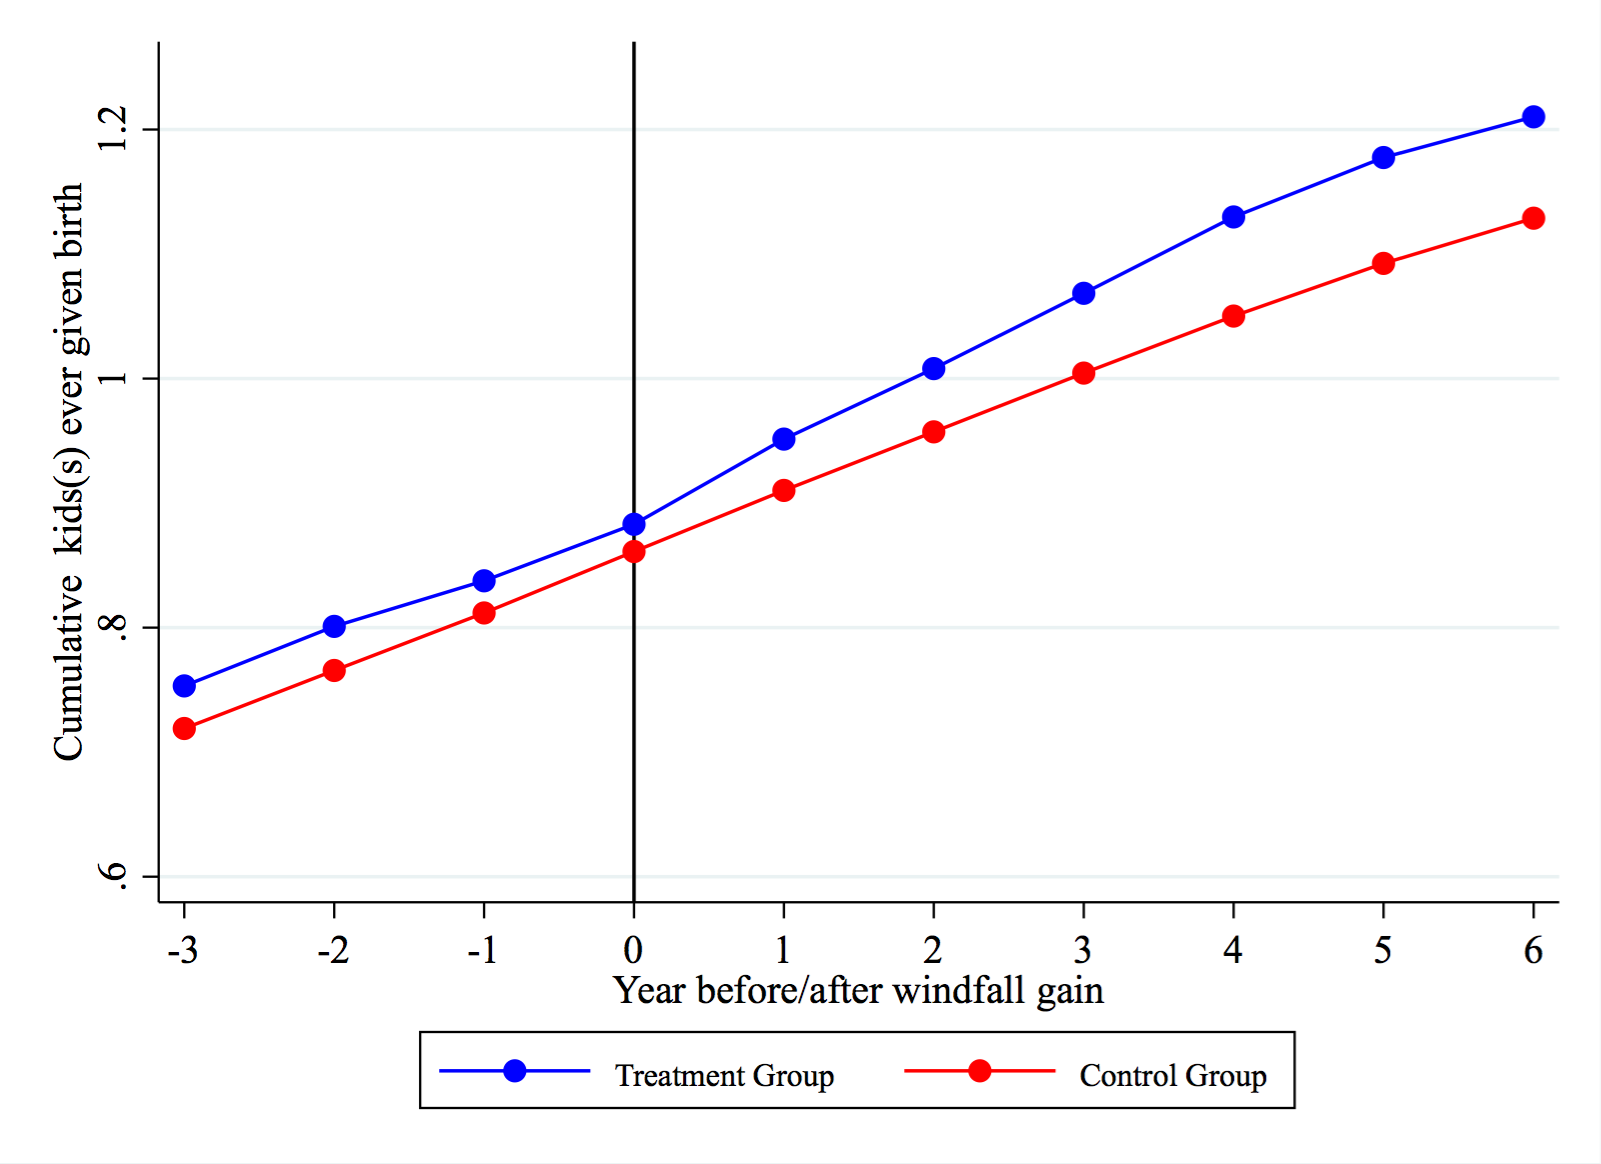
\includegraphics[width=1.0\textwidth]{figure/totbaby.png} 
	%\begin{itemize}
	%\hyperlink{sub_2}{\beamergotobutton{back}} 
	%\end{itemize}
\end{frame}



\begin{frame}{Examining Parallel Pre-Trends}{Raw Data: Cumulative Number of Children}
		\begin{itemize} 
		\item Since we focus on trend rather than level, we sometimes subtract the baseline mean ($k=-1$) from the outcome at each time period 
		\end{itemize}
	
\end{frame}


\begin{frame}{Examining Parallel Pre-Trends}{Subtract the Baseline Mean: Cumulative Number of Children}
	
	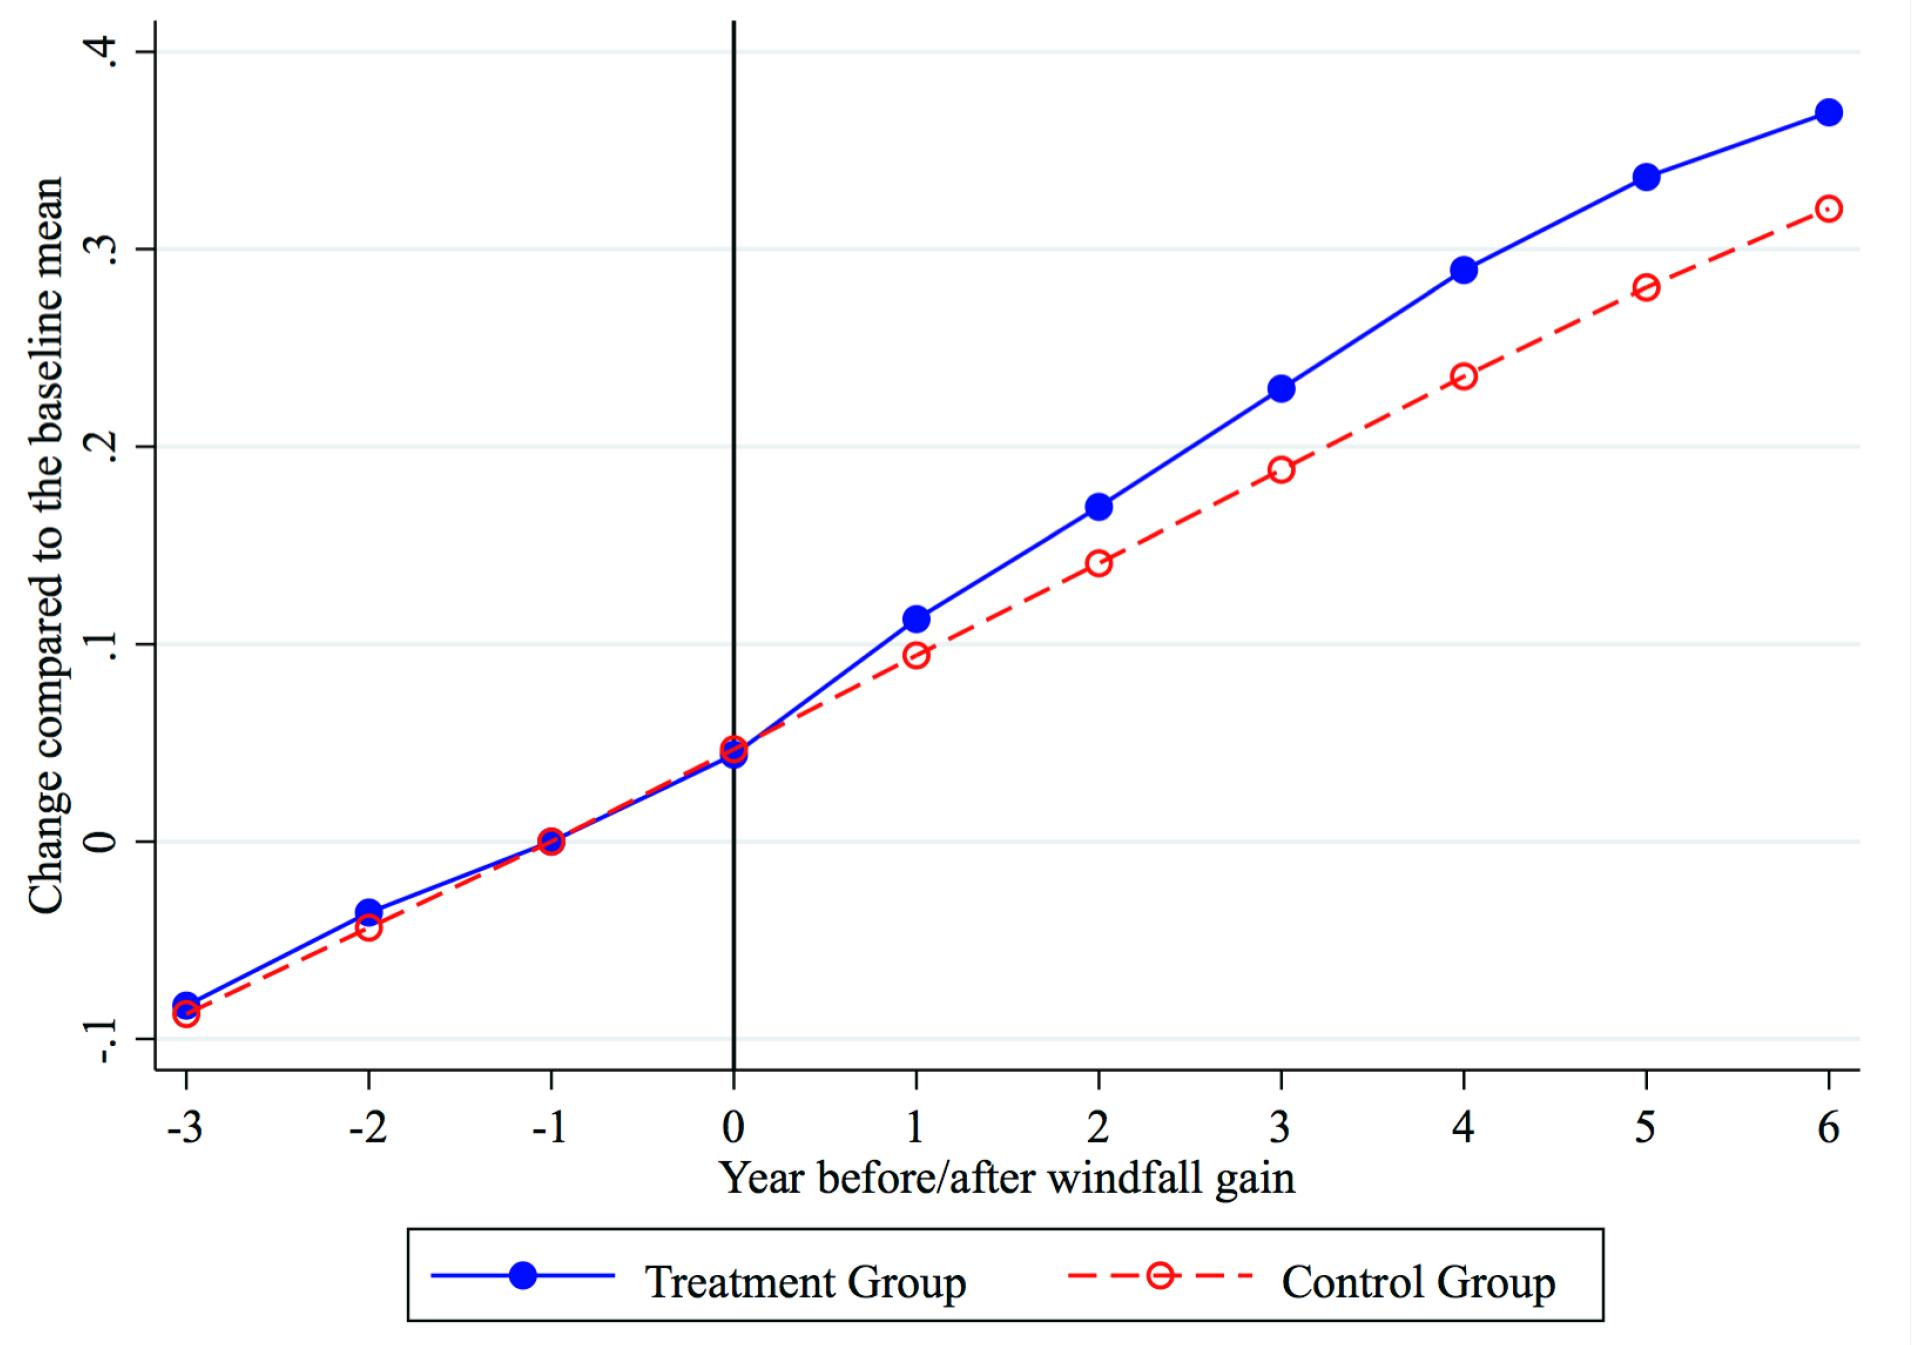
\includegraphics[width=1.0\textwidth]{figure/child_f1.jpg} 
	%\begin{itemize}
	%\hyperlink{sub_2}{\beamergotobutton{back}} 
	%\end{itemize}
\end{frame}




\begin{frame}{Examining Parallel Pre-Trends}{Raw Data: Cumulative Number of Children}
	\begin{itemize} 
		\item We can formally examine whether two groups share similar pre-treatment trend by showing the estimated coefficients $\gamma_{-2}, \gamma_{-3},...,\gamma_{6} $
					\vspace{0.3cm}
	\item If pre-treatment trend is parallel between two groups, $\gamma_{-2}, \gamma_{-3}$ should be close to zero
	\vspace{0.3cm}
	\item $\gamma_{0}, \gamma_{1},...,\gamma_{6} $ represent the treatment effects of winning lotteries 
	\end{itemize}
	
\end{frame}



\begin{frame}{Examining Parallel Pre-Trends}{Dynamic DID design: Cumulative Number of Children}
	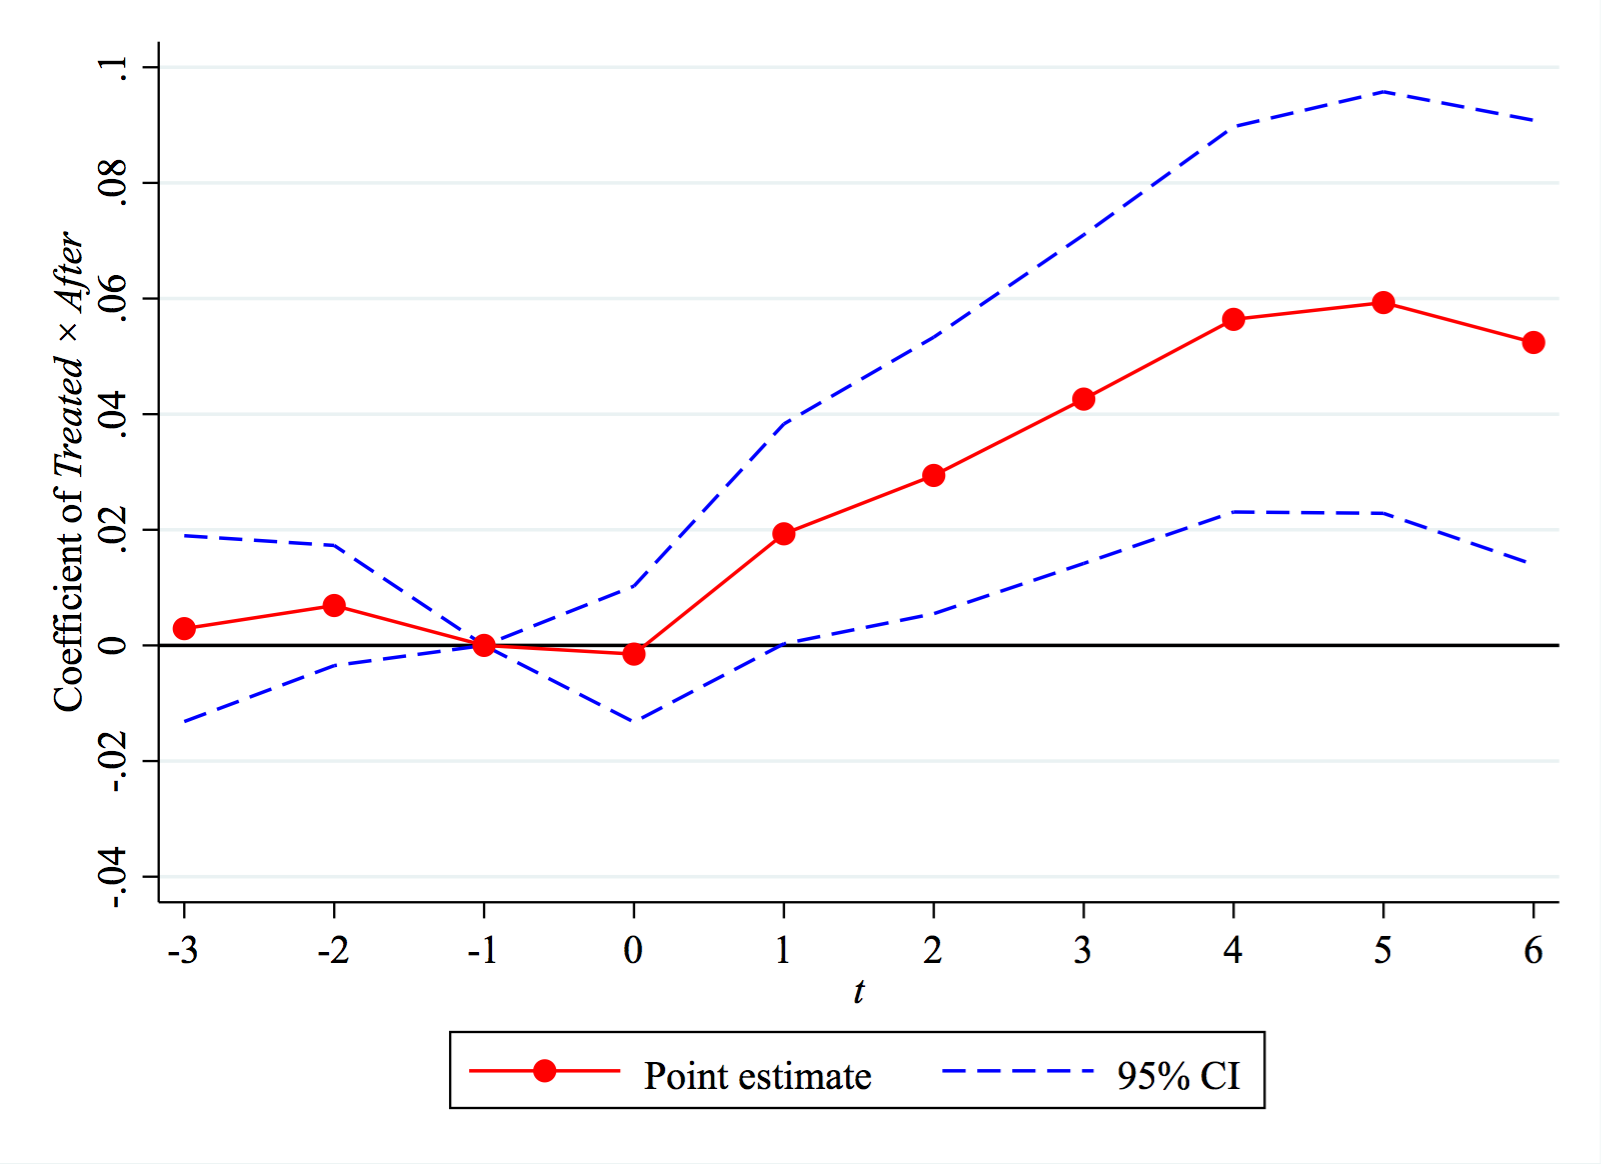
\includegraphics[width=1.0\textwidth]{figure/totbaby_e.png} 
	%\begin{itemize}
	%\hyperlink{sub_2}{\beamergotobutton{back}} 
	%\end{itemize}
\end{frame}



\begin{frame}{Another Way to Examine Parallel Pre-Trends}{}
	\begin{itemize}
		\item Conduct a DID estimation using pre-treatment data
		\vspace{0.2cm}
		\item Arbitrarily choose a ``treatment timing" in the pre-treatment period 
		
		
\begin{equation*}
	Y_{it}=\mu+ \gamma D_i+ \delta Placebo_t+ \alpha (D_i\times Placebo_t)+X'_{it}\beta+\varepsilon_{it},
\end{equation*}		
		
		\item $Placebo$ is a dummy indicating fake ``post-treatment" period
		
		\item If pre-trend is parallel between two groups, we would expect $\alpha=0$
	\end{itemize}
	
	
	
	
\end{frame}




\title[]  
{STATA Example}


\author 
{}

%\institute{Institute of Economics, Academia Sinica  \\ Econ, NTU}
%\institute{Institute of Economics, Academia Sinica  \\ IMES/IDAS, NCCU}
\institute{}

%\author 
%{楊子霆 \\ 中研院經濟所}

%\institute 
%{中正大學國際經濟專題研討}




\date
{}


\begin{frame}{}
\titlepage
\end{frame}





\begin{frame}{Empirical Example 1: Eissa and Jeffrey (1996)}
Eissa, Nada, and Jeffrey B. Liebman. (1996) ``\textbf{Labor Supply Responses to the Earned Income Tax Credit}" QJE
\begin{itemize}
\vspace{0.2cm}
\item They want to look at the effect of tax credit on labor supply


\end{itemize}
\end{frame}



\begin{frame}{Empirical Example 1: Eissa and Jeffrey (1996)}{STATA Implementation}
\begin{itemize}
\item See DID.do
\vspace{0.2cm}
\item Use eitc.dta


\end{itemize}
\end{frame}





\begin{frame}{Empirical Example 1: Eissa and Jeffrey (1996)}
\begin{itemize}
\item Earned Income Tax Credit (EITC) is a refundable tax credit that subsidizes earnings of working poor in US
\vspace{0.2cm} 
\begin{itemize}
\item The amount of cash transfer depends on the number of children and previous year earnings
\vspace{0.2cm}
\item In 1994, the amount of EITC had large increase for those who have children
\vspace{0.2cm}
\end{itemize}
\item The author examined how did labor supply respond to this change in tax credit using DID design

\end{itemize}
\end{frame}


\begin{frame}{EITC benefit rule}
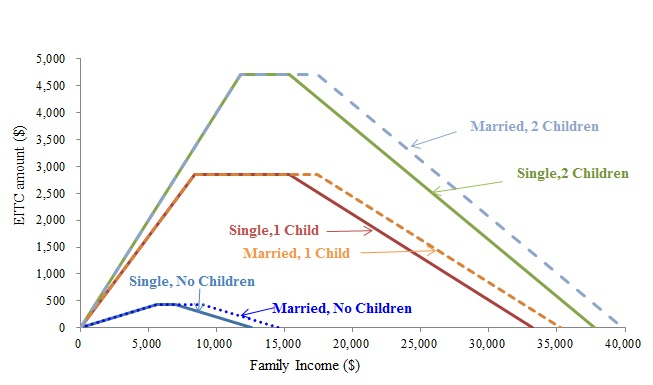
\includegraphics[width=0.9\textwidth]{figure/eitc_pict_6R_2.jpg} 
\end{frame}



\begin{frame}{Step 1: Define treatment and control groups}
\begin{itemize}
%\item The first step of DID analysis is to define treatment and control groups 
%\vspace{0.2cm}
%\begin{itemize}		
\item Treatment group: those who have at least one children 
\vspace{0.2cm}		
\begin{itemize}		
\item They receive much more tax credit after 1994
\vspace{0.2cm}				
\end{itemize}
\item Control group: those who do not have children 
\vspace{0.2cm}	

\begin{itemize}		
\item Their tax credit did not increase after 1994		
\end{itemize}		
\end{itemize}	


%\end{itemize}
\end{frame}




\begin{frame}{Step 1: Define treatment and control groups}
\begin{itemize}

\item $D$: a dummy that indicate whether individual $i$ had children or not 
\begin{align*}
D=\left\lbrace
\begin{array}{l}
1\quad \text{if individual $i$ had at least one children}\\
0\quad \text{if individual $i$ did not have children}
\end{array} \right.
\end{align*}


\end{itemize}
\end{frame}










\begin{frame}{Step 1: Define treatment and control groups}
\begin{itemize}
\item $Post$: a dummy that indicate whether individual $i$ was observed after 1994 (Post-treatment period)
\begin{align*}
Post=\left\lbrace
\begin{array}{l}
1\quad \text{if individual $i$ was observed after 1994}\\
0\quad \text{if individual $i$ was observed before 1994}
\end{array} \right.
\end{align*}
\item $D \times Post$: a treatment dummy that indicate whether individual $i$ was affected by 1994 EITC expansion

\end{itemize}
\end{frame}



\begin{frame}[fragile]{Step 1: Define treatment and control groups}{STATA Command}


\begin{lstlisting}
** a dummy for treatment group
gen treated = (children >= 1)

** a dummy for post-treatment period
gen post = (year >= 1994)

** treatment variable (DID key variable)
gen treated_post = treated*post
\end{lstlisting}
\begin{itemize}
\item Create dummy variables for treatment group, post-treatment period and treatment variable (DID) 

\end{itemize}
\end{frame}





\begin{frame}{Step 2: Graphical Analysis}
\begin{itemize}
\item Plot the time trend of outcomes for treatment and control groups 
\vspace{0.2cm}
\begin{itemize}
\item Check whether there is a \textbf{parallel trend} in outcomes of treatment and control groups \textbf{before reform}
\vspace{0.2cm}
\item Examine whether the outcomes of treatment group exhibits different trend \textbf{after reform}
\end{itemize}
\end{itemize}
\end{frame}


\begin{frame}[fragile]{Step 2: Graphical Analysis}{STATA Command}

\begin{lstlisting}
collapse (mean) work, by(year treated)
\end{lstlisting}
\vspace{0.2cm}
\begin{itemize}
\item \textbf{collapse:} This command converts the data into a dataset of summary statistics, such as sums, means, medians, and so on
\vspace{0.2cm}
\begin{itemize}
\item Converts the data into mean of ``work" (Labor Force Participation Rates) by group and year - group and year mean
\end{itemize}

\end{itemize}
\end{frame}





\begin{frame}[fragile]{Step 2: Graphical Analysis}{STATA Command}
\begin{lstlisting}			
graph twoway (line work year if treated==0) (line work year if treated==1), legend(order(1 "Control Group" 2 "Treatment Group")) ///
graphregion(fcolor(white) lcolor(white) ifcolor(white) ilcolor(white)) ///
xline(1994, lp(dash) lc(black) lw(medthin)) ///
ytitle(Labor Force Participation Rates)
\end{lstlisting}
\begin{itemize}
\item Create a twoway gragh ("work" by "year") for treatment and control groups
\end{itemize}
\end{frame}



\begin{frame}{Trend in Outcomes for Treatment and Control Groups}

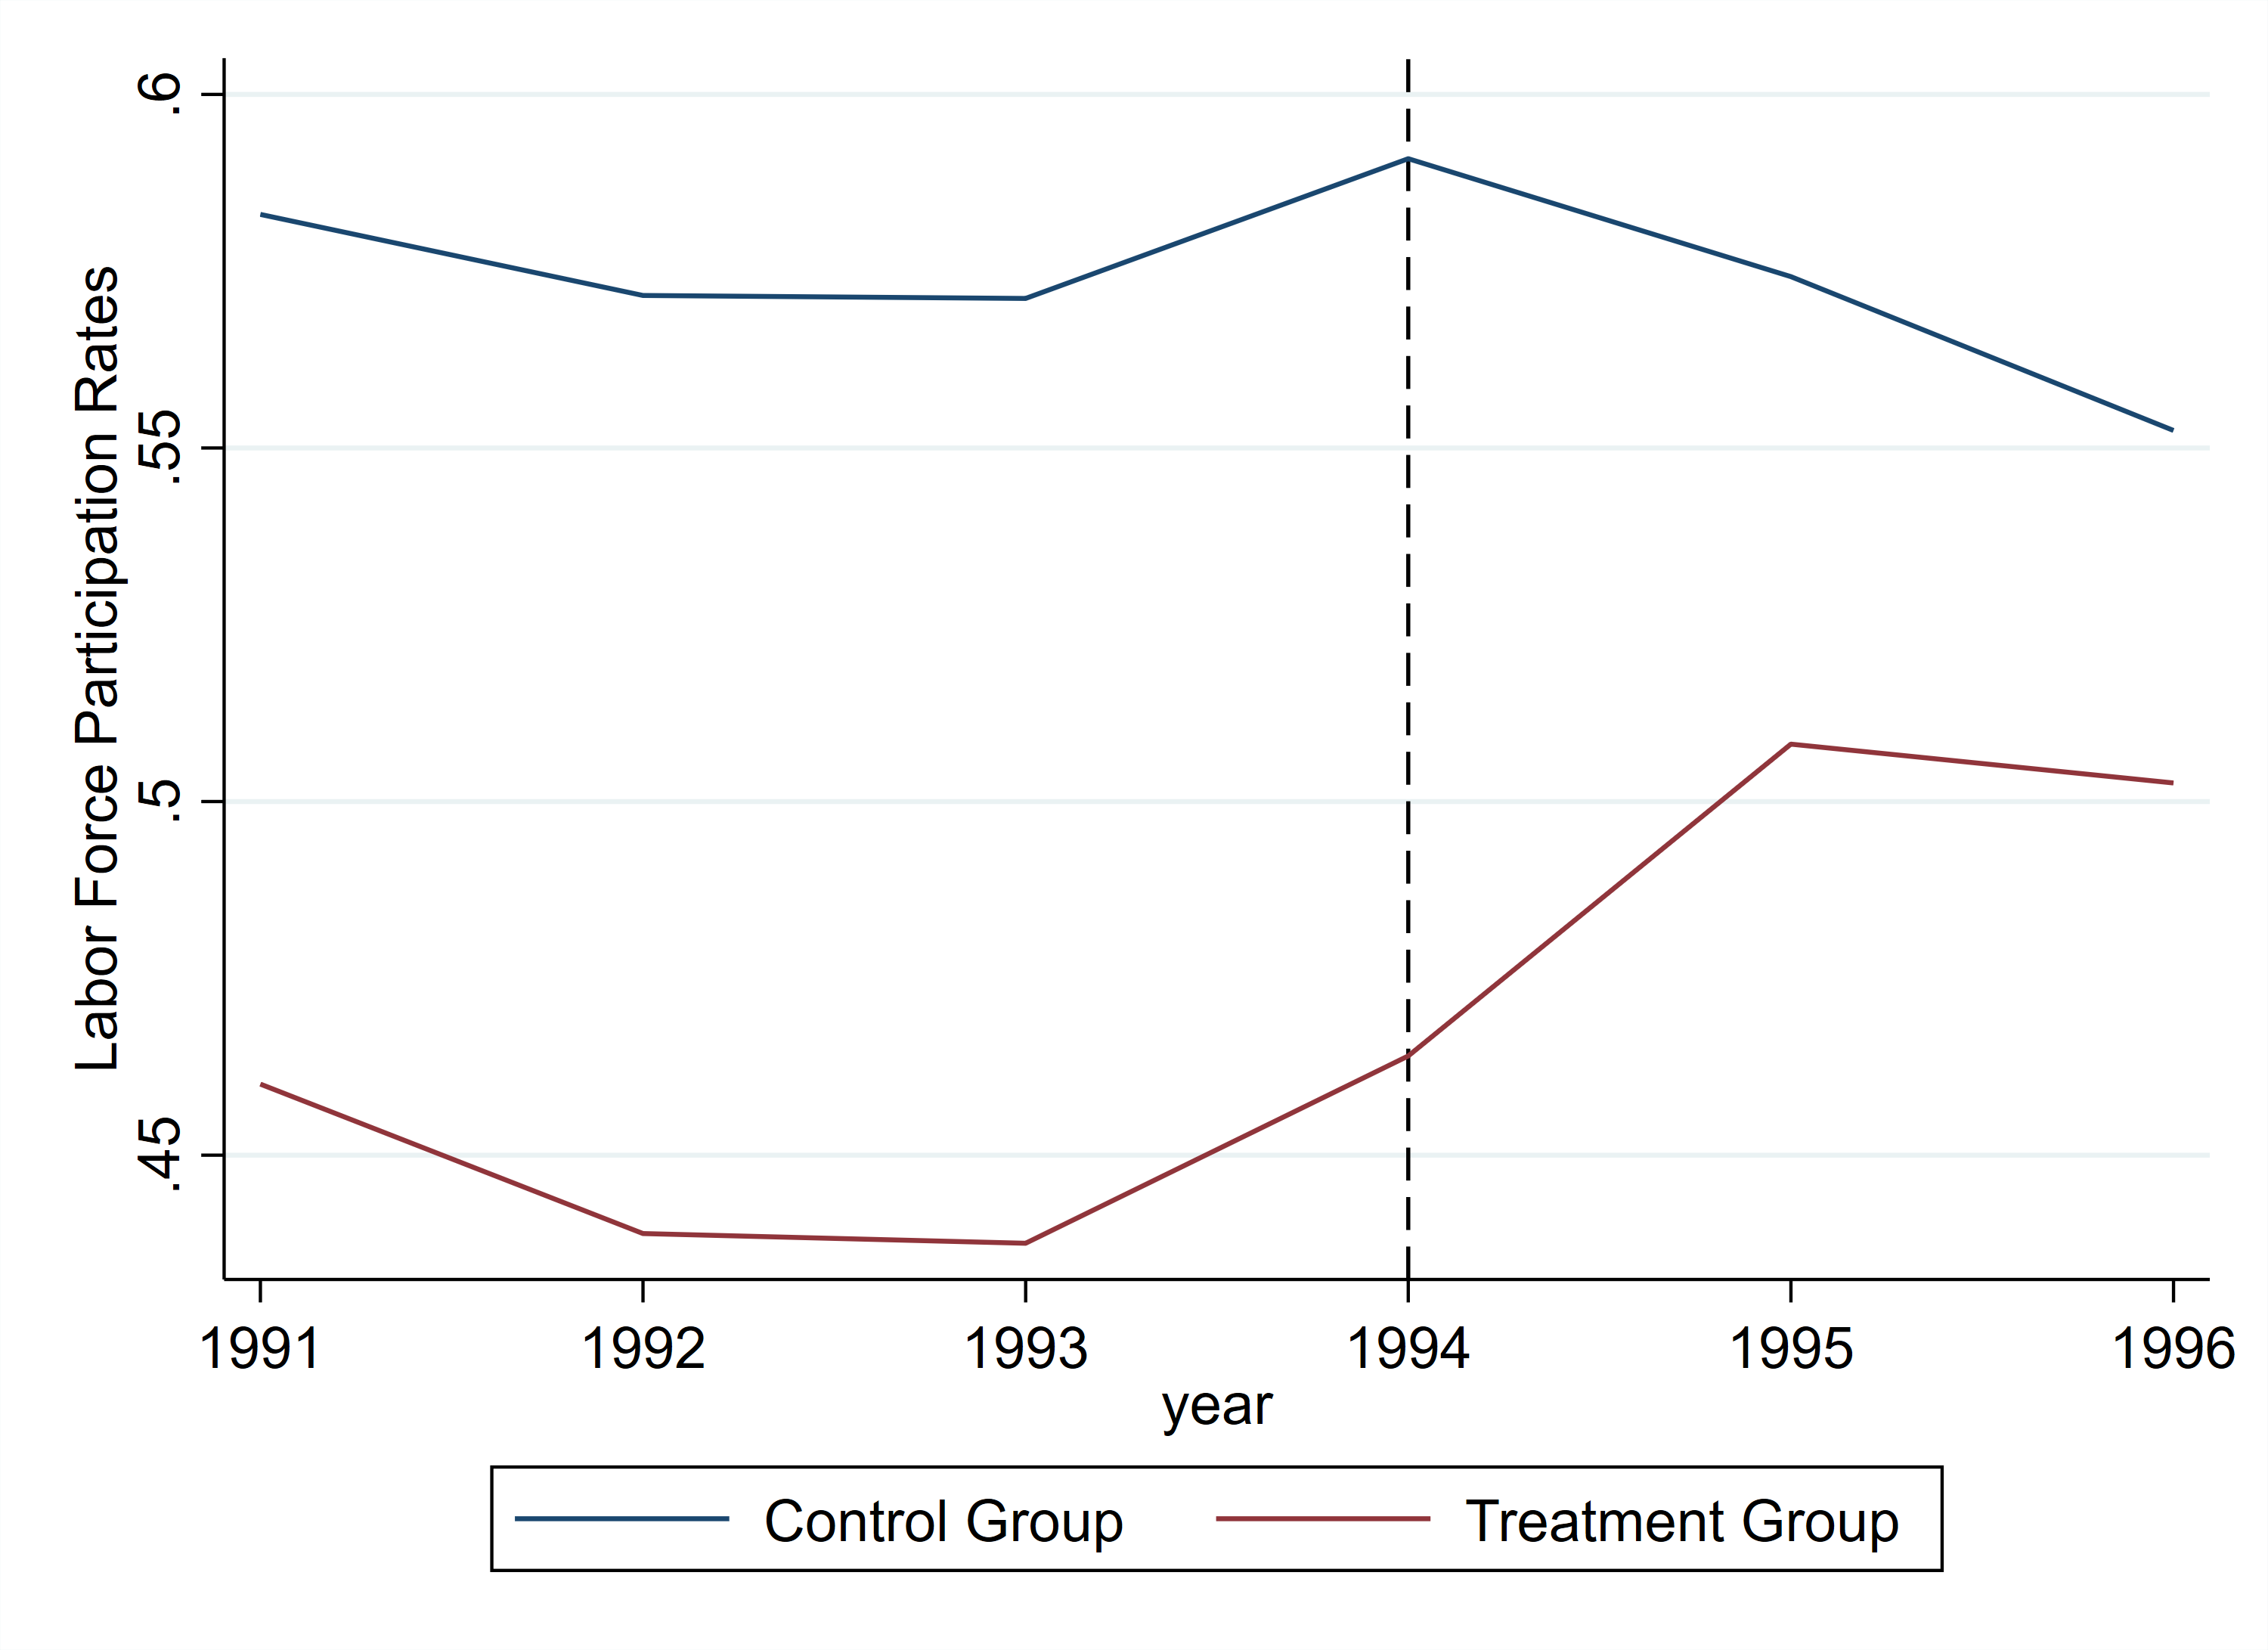
\includegraphics[width=0.9\textwidth]{figure/eitc_DID.png}


\end{frame}



\begin{frame}[fragile]{Step 3: Pre/Post DID regression}{STATA Command}
\begin{itemize}
\item We can estimate the following DID regression:
\begin{equation*}
Y_{it}=\mu+ \gamma D_i+ \delta Post_t+ \alpha (D_i\times Post_t)+X'_{it}\beta+\varepsilon_{it},
\end{equation*}
\end{itemize}
\end{frame}


% ---------- outreg2 ----------
\begin{frame}[fragile]{Step 3: Pre/Post DID regression}{STATA: \texttt{outreg2} $\to$ .tex}
\begin{lstlisting}
reg work post treated treated_post, r
outreg2 using "$table\DID_pre_post.tex", replace nocon ///
    keep(treated_post) stats(coef se) label            ///
    addstat(Observations, e(N)) ctitle("(1)")          ///
    addtext(Age, , Demo, , State FE, , Year FE, )

* Cols (2)-(5): replace -> append; update addtext() per column
\end{lstlisting}
\begin{itemize}
    \item \textbf{replace} for col~(1); \textbf{append} for cols~(2)--(5)
    \vspace{0.15cm}
    \item \textbf{addtext()}: control indicator rows must be filled \textbf{manually} for every column
    \vspace{0.15cm}
    \item Output uses \texttt{\textbackslash hline} (not booktabs); ``Yes''/``'' labels only — no $\surd$ support
\end{itemize}
\end{frame}

% ---------- esttab: code ----------
\begin{frame}[fragile]{Step 3: Pre/Post DID regression}{STATA: \texttt{esttab} $\to$ .tex (code)}
\begin{lstlisting}
* ssc install estout  (run once)
local surd = char(36) + "\surd" + char(36)

eststo clear
eststo m1: reg work post treated treated_post, r
eststo m2: reg work post treated treated_post age age2, r
* (m3: +demographics  m4: +state FE  m5: +year FE)
eststo m5: reg work post treated treated_post ///
    nonwhite age age2 ed finc nonlaborinc i.state i.year, r

esttab m1 m2 m3 m4 m5 using "$table\DID_pre_post.tex", replace ///
    booktabs keep(treated_post) label                           ///
    mtitles("(1)" "(2)" "(3)" "(4)" "(5)") nonumbers            ///
    stats(N, fmt(%9.0fc) labels("Observations"))                ///
    star(* 0.10 ** 0.05 *** 0.01) b(%9.3f) se par              ///
    indicate("Age Controls = age age2"                          ///
             "Demographics = nonwhite ed finc nonlaborinc"      ///
             "State FE = *.state" "Year FE = *.year",           ///
             labels("`surd'" ""))
\end{lstlisting}
\end{frame}

% ---------- esttab: options ----------
\begin{frame}{Step 3: Pre/Post DID regression}{STATA: \texttt{esttab} $\to$ .tex (options)}
\begin{itemize}
    \item \textbf{eststo m1: reg \ldots}: stores results; \textbf{esttab} combines all into one table
    \vspace{0.2cm}
    \item \textbf{booktabs}: replaces \texttt{\textbackslash hline} with
          \texttt{\textbackslash toprule / \textbackslash midrule / \textbackslash bottomrule}
          --- matches publication style
    \vspace{0.2cm}
    \item \textbf{indicate()}: \textbf{auto-detects} which variables are in each model
          and inserts $\surd$ or blank --- no manual filling needed
    \vspace{0.2cm}
    \item \textbf{char(36)}: Stata trick for a literal \texttt{\$} sign
          (``\texttt{\$\textbackslash surd\$}'' triggers macro expansion; use
          \texttt{char(36) + "\textbackslash surd" + char(36)} instead)
\end{itemize}
\end{frame}









\begin{frame}{Pre/Post DID Results}
\vspace{-0.2cm}
\begin{table}[h]
\centering
\footnotesize
\caption{Effect of EITC Expansion on Labor Force Participation}
\begin{tabular}{@{}lccccc@{}}
\toprule
 & (1) & (2) & (3) & (4) & (5) \\
\midrule\midrule
Treat $\times$ Post & 0.047*** & 0.041*** & 0.046*** & 0.046*** & 0.045*** \\
                   & (0.011)  & (0.011)  & (0.010)  & (0.010)  & (0.010)  \\
\midrule\midrule
Observations       & \multicolumn{5}{c}{13,746} \\
\midrule\midrule
Age Controls       &          & $\surd$  & $\surd$  & $\surd$  & $\surd$  \\
Demographics       &          &          & $\surd$  & $\surd$  & $\surd$  \\
State FE           &          &          &          & $\surd$  & $\surd$  \\
Year FE            &          &          &          &          & $\surd$  \\
\bottomrule
\end{tabular}
\end{table}
{\tiny Robust SE in parentheses. *** p$<$0.01, ** p$<$0.05, * p$<$0.1.}


\end{frame}

\begin{frame}[fragile]{Step 3: Pre/Post DID regression}{STATA Command}
\begin{itemize}
\item Show the treatment effect by treatment intensity:
\begin{lstlisting}	
** treatment intensity
gen treated_1 = (children==1) 
gen treated_2 = (children>=2)
gen treated_post_1 = post*treated_1
gen treated_post_2 = post*treated_2

reg work post treated_1 treated_2 treated_post_1 treated_post_2 nonwhite age age2 ed finc nonlaborinc,r
\end{lstlisting}
\end{itemize}
\end{frame}


\begin{frame}{Pre/Post DID Results}{Treatment Intensity}

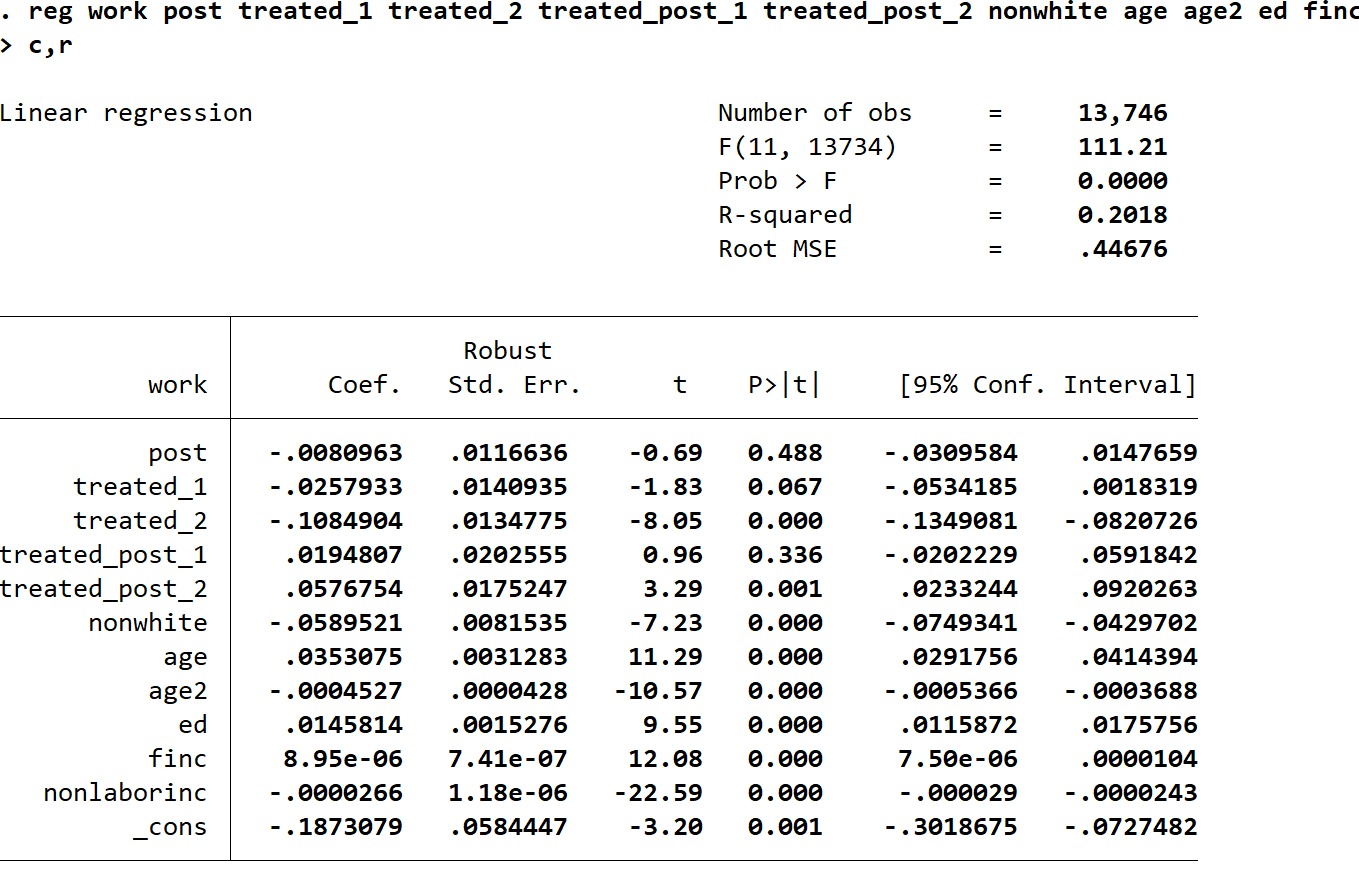
\includegraphics[width=1.0\textwidth]{figure/stata_did_table2.png}


\end{frame}



\begin{frame}[fragile]{Step 4: Examine Common Trend by a Placebo Test}{STATA Command}
\begin{itemize}
\item Creating a placebo DID model is when you arbitrarily choose a treatment time before your actual treatment time
\vspace{0.2cm}
\item Test to see if you get a "significant" treatment effect (Hope not)

\begin{lstlisting}	
gen placebo = (year >= 1992)
gen treated_placebo = treated*placebo

reg work treated placebo treated_placebo if year<1994,r
\end{lstlisting}
\end{itemize}
\end{frame}


\begin{frame}{Placebo Test}

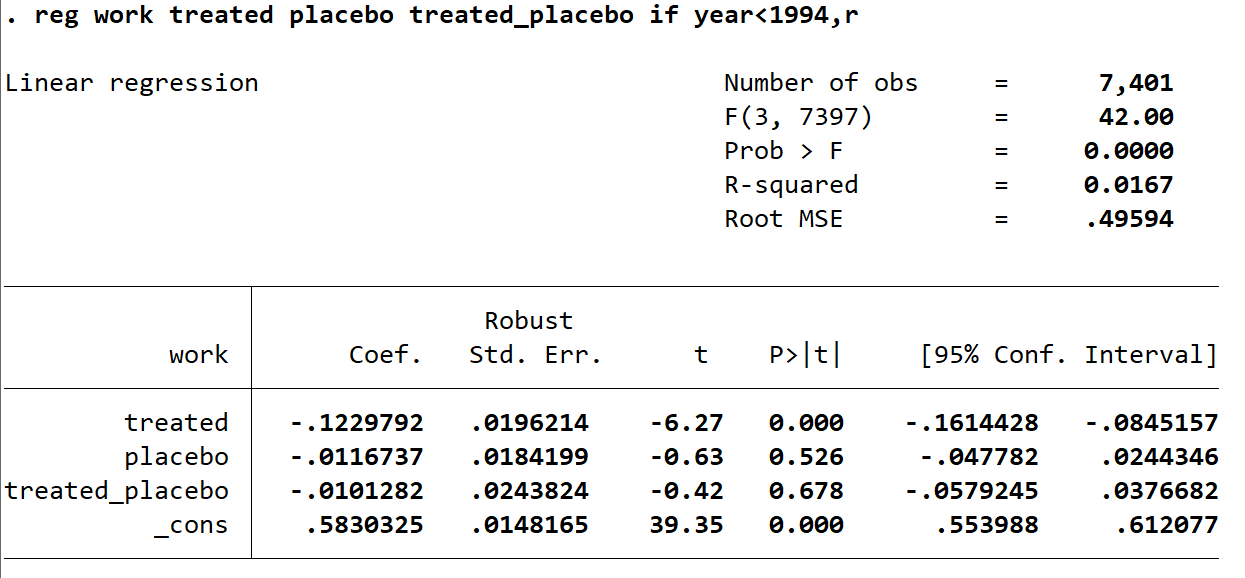
\includegraphics[width=1.0\textwidth]{figure/stata_did_table4.png}


\end{frame}





\begin{frame}[fragile]{Step 5: Dynamic DID Design}{STATA Command}
\begin{lstlisting}	
reg work treated pre_event_3 pre_event_2 post_event_0-post_event_2 pre_dd_3 pre_dd_2 post_dd_0 -post_dd_2 nonwhite age age2 ed finc nonlaborinc,r

outreg2 using "$table\DID_dynamic.xls", replace nocon keep(pre_dd_* post_dd_*)
 year<1994,r
\end{lstlisting}
\end{frame}


\begin{frame}{Dynamic DID Estimates}
	
	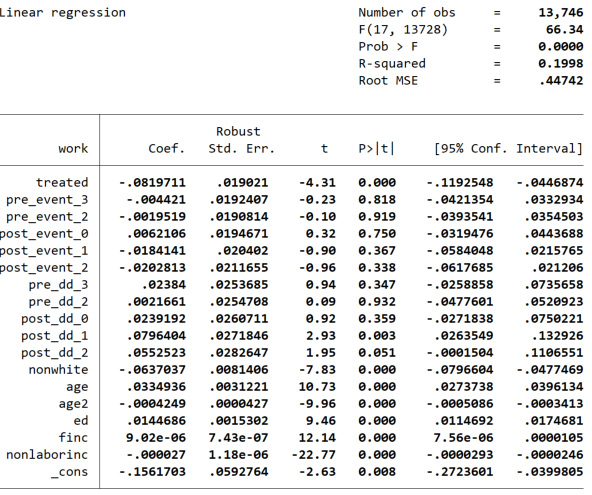
\includegraphics[width=1.0\textwidth]{figure/stata_did_table5.png}
	
	
\end{frame}



\begin{frame}{Dynamic DID Estimates}{Graph}
	
	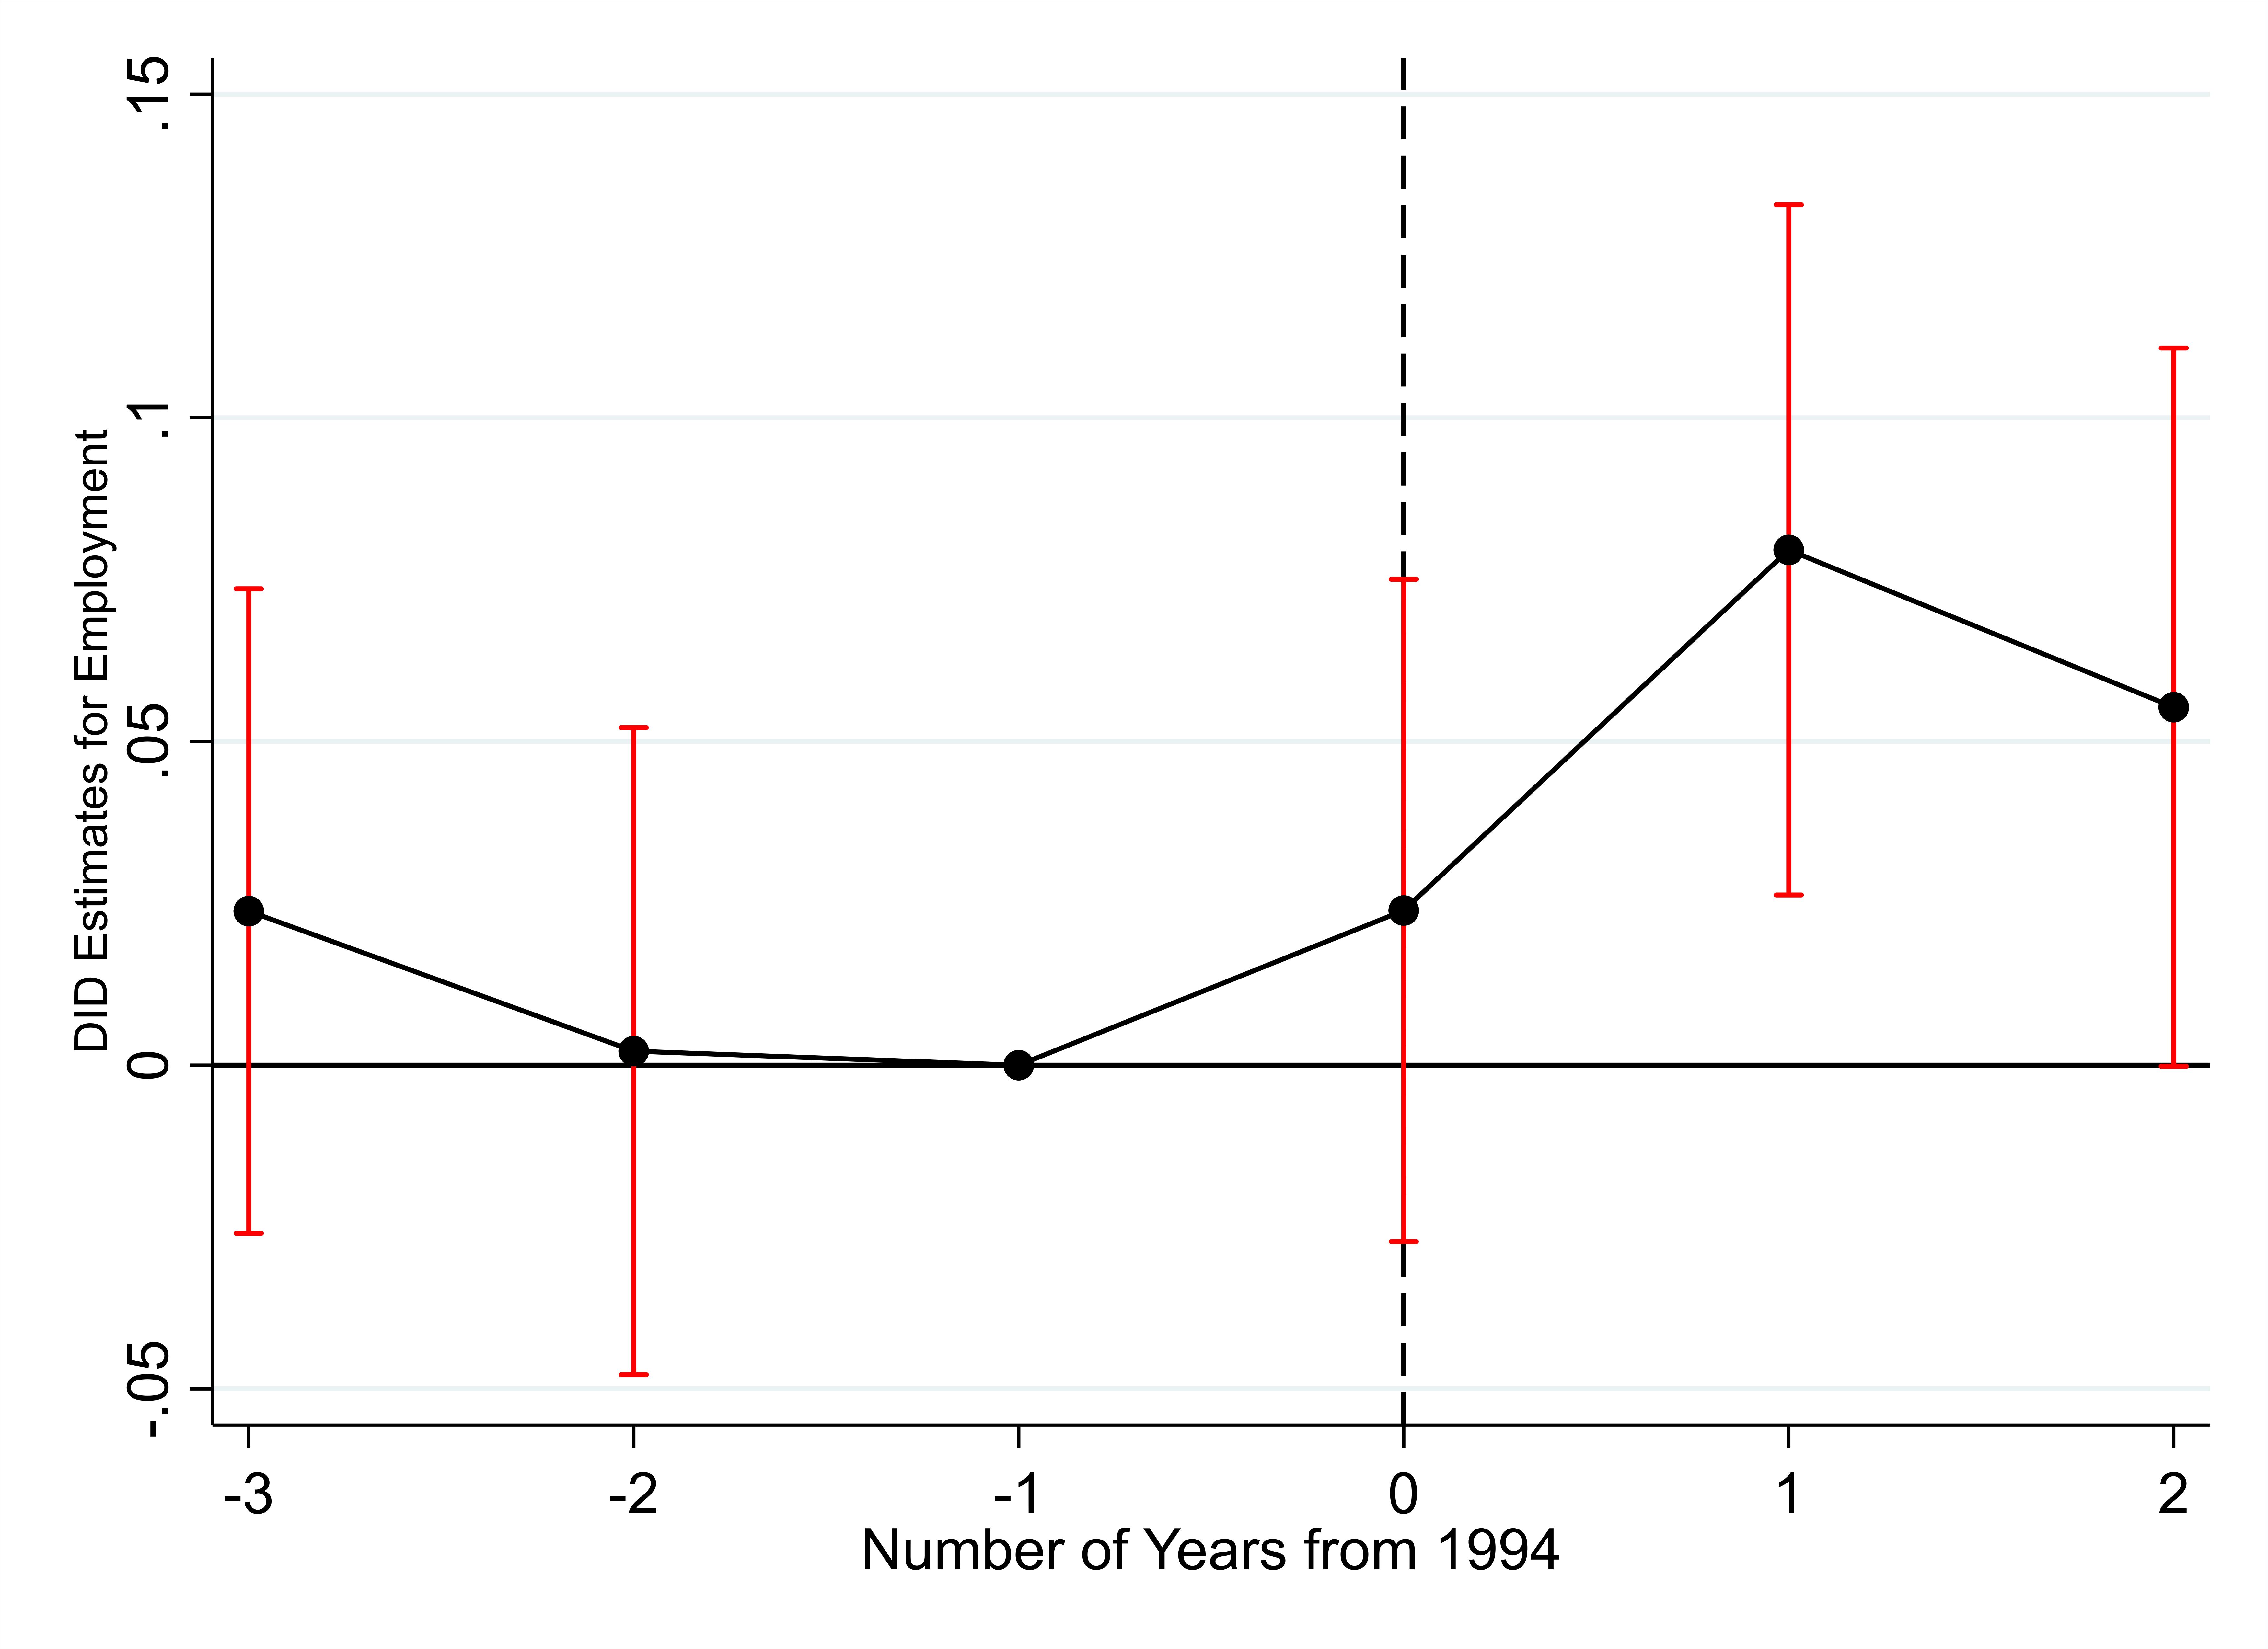
\includegraphics[width=0.9\textwidth]{figure/DID_dynamic.png}
	
	
\end{frame}







\title[]  
{R Example}


\author 
{}

%\institute{Institute of Economics, Academia Sinica  \\ Econ, NTU}
%\institute{Institute of Economics, Academia Sinica  \\ IMES/IDAS, NCCU}
\institute{}

%\author 
%{楊子霆 \\ 中研院經濟所}

%\institute 
%{中正大學國際經濟專題研討}




\date
{}


\begin{frame}{}
	\titlepage
\end{frame}






\begin{frame}[fragile]{Step 1: Define treatment and control groups}{R Command}

\begin{lstlisting}
eitc_data <- eitc_data %>%
mutate(treated = as.numeric(children >= 1),
post = as.numeric(year >= 1994),
treated_post = treated * post,
age2 = age^2,  
nonlaborinc = finc - earn)  
\end{lstlisting}
	\begin{itemize}

\item \textbf{\%>\%:} The pipe operator passes the data from the left side to the function on the right side as the first argument, 
	\vspace{0.2cm}
	\begin{itemize}
\item Allowing for more readable code by chaining operations sequentially
	\end{itemize}
	\vspace{0.2cm}
\item \textbf{as.numeric():} Converts logical values (TRUE/FALSE) to numeric values (1/0)

	\end{itemize}
\end{frame}


\begin{frame}[fragile]{Step 2: Graphical Analysis}{R Command}

\begin{lstlisting}
data_summary <- eitc_data %>%
group_by(year, treated) %>%
summarise(work_mean = mean(work, na.rm = TRUE))
\end{lstlisting}

\begin{itemize}
\item \textbf{data\_summary:} Create a summary of the dataset for graphical analysis.
\begin{itemize}
	\item \textbf{group\_by(year, treated):} Groups the data by year and treatment status.
	\vspace{0.2cm}
	\item \textbf{summarise(work\_mean = mean(work, na.rm = TRUE)):} Calculates the mean work participation for each group, ignoring missing values.
\end{itemize}


\end{itemize}
\end{frame}



\begin{frame}[fragile]{Step 2: Graphical Analysis}{R Command}
\begin{lstlisting}
ggplot(data_summary, aes(x = year, y = work_mean, color = factor(treated))) +
geom_line(size = 1) +
scale_color_manual(values = c("blue", "red"),
labels = c("Control Group", "Treatment Group")) +
geom_vline(xintercept = 1994, linetype = "dashed", color = "black") +
labs(title = "Labor Force Participation Rates",
y = "Labor Force Participation Rates",
color = "Group") +
theme_minimal() +
theme(legend.position = "top",
panel.grid.major = element_blank(),
panel.grid.minor = element_blank())

ggsave(paste0(pic, "/eitc_DID.png"), width = 12, height = 8, units = "in")
\end{lstlisting}
\end{frame}



\begin{frame}{DID graph}
	
	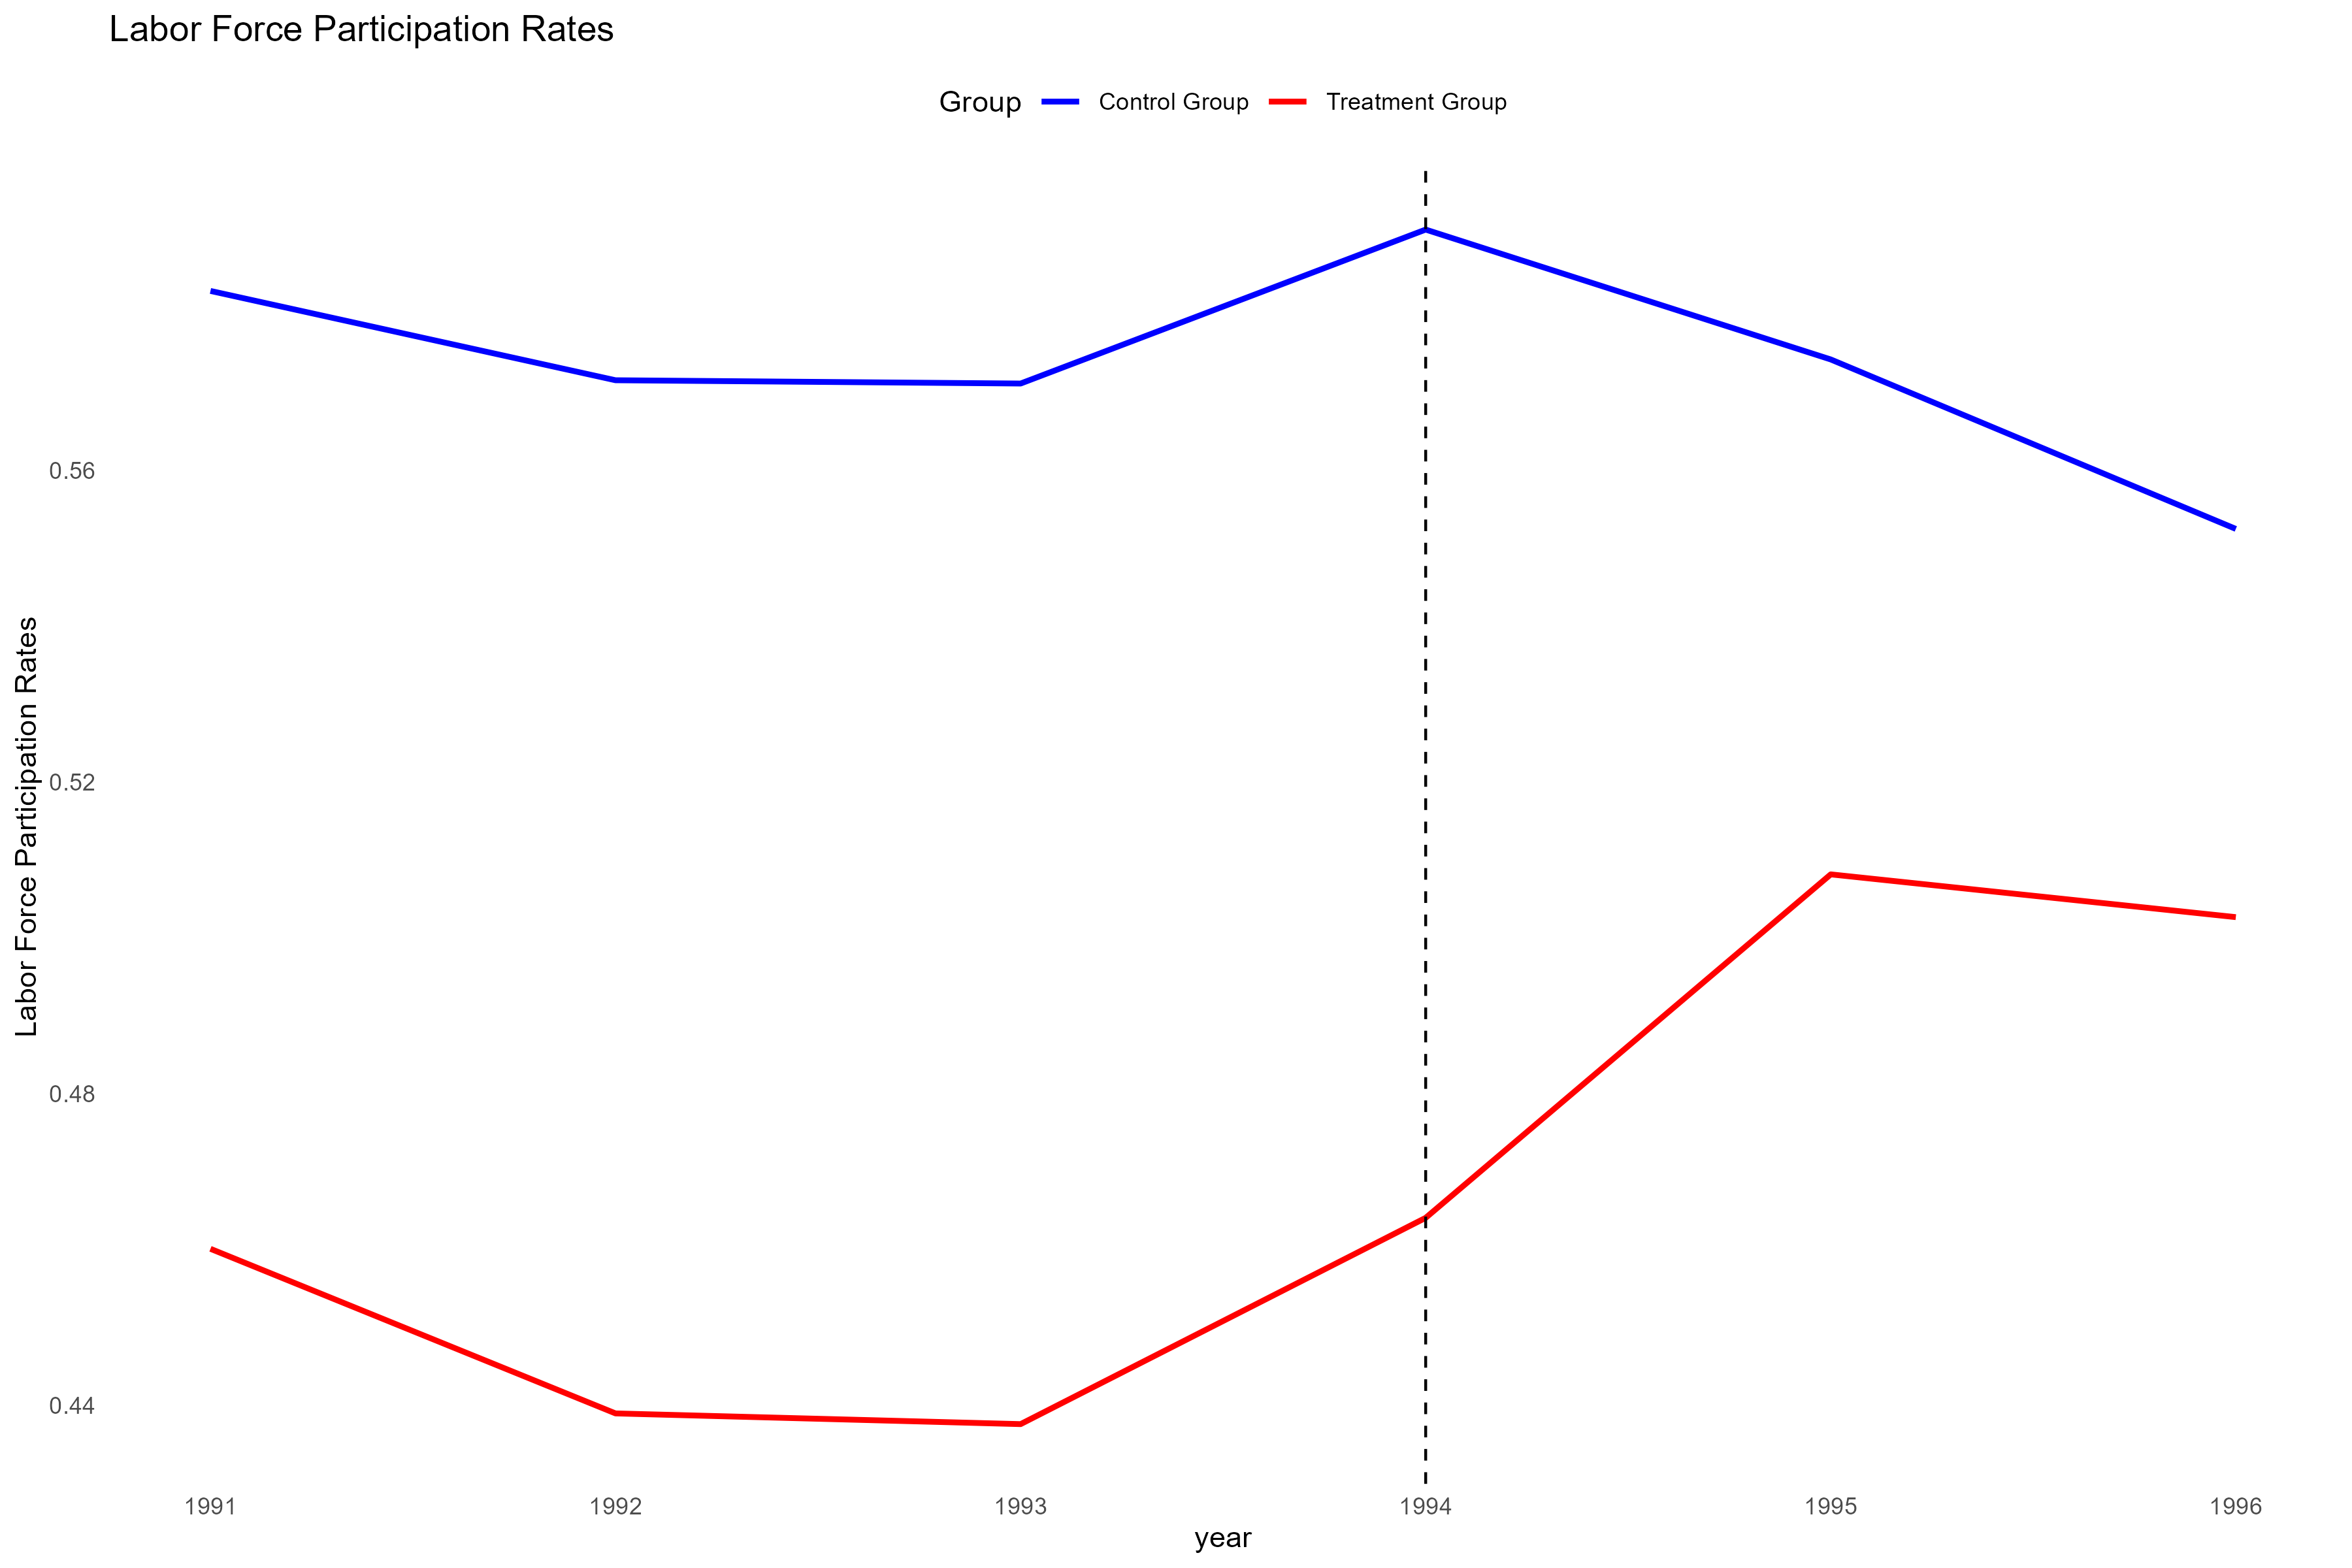
\includegraphics[width=1.0\textwidth]{figure/eitc_did_R.png}
	
	
\end{frame}









% ---------- modelsummary 1/3: backend fix ----------
\begin{frame}[fragile]{Step 3: Pre/Post DID regression}{R: \texttt{modelsummary} $\to$ .tex (1/3)}
\begin{itemize}
    \item \textbf{modelsummary 2.0+} defaults to \textbf{tinytable} backend, which outputs
          tex requiring \texttt{tabularray}, \texttt{siunitx}, \ldots\
          --- incompatible with standard Beamer/\LaTeX
    \vspace{0.15cm}
    \item Fix: force \textbf{kableExtra} backend \textbf{before} calling \texttt{modelsummary}
\end{itemize}
\begin{lstlisting}
options("modelsummary_factory_latex"        = "kableExtra")
options("modelsummary_format_numeric_latex" = "plain")
library(kableExtra)

ck <- "$\\surd$"      # LaTeX checkmark — no $-macro issue in R
models_list <- list("(1)"=model1, "(2)"=model2, "(3)"=model3,
                    "(4)"=model4, "(5)"=model5)
\end{lstlisting}
\end{frame}

% ---------- modelsummary 2/3: code ----------
\begin{frame}[fragile]{Step 3: Pre/Post DID regression}{R: \texttt{modelsummary} $\to$ .tex (2/3)}
\begin{lstlisting}
rows <- data.frame(
  term=c("Age Controls","Demographics","State FE","Year FE"),
  `(1)`=c("","","",""), `(2)`=c(ck,"","",""),
  `(3)`=c(ck,ck,"",""), `(4)`=c(ck,ck,ck,""),
  `(5)`=c(ck,ck,ck,ck), check.names=FALSE)

modelsummary(models_list,
  coef_map = c("treated_post" = "Treat $\\times$ Post"),
  gof_map  = list(list("raw"="nobs","clean"="Observations","fmt"=0)),
  stars    = c("*"=0.1,"**"=0.05,"***"=0.01),
  add_rows = rows,
  booktabs = TRUE,
  output   = file.path(table, "DID_pre_post.tex"))
\end{lstlisting}
\end{frame}

% ---------- modelsummary 3/3: options ----------
\begin{frame}{Step 3: Pre/Post DID regression}{R: \texttt{modelsummary} $\to$ .tex (3/3)}
\begin{itemize}
    \item \textbf{coef\_map}: renames + selects coefficients ---
          only \texttt{treated\_post}, labelled ``Treat $\times$ Post''
    \vspace{0.2cm}
    \item \textbf{gof\_map}: selects GOF stats ---
          only \texttt{nobs} displayed as ``Observations''
    \vspace{0.2cm}
    \item \textbf{add\_rows}: appends custom rows (control indicators) at the bottom
    \vspace{0.2cm}
    \item \textbf{booktabs = TRUE}: \texttt{\textbackslash toprule / \textbackslash midrule / \textbackslash bottomrule}
          --- same as \texttt{esttab}'s \texttt{booktabs} option
    \vspace{0.2cm}
    \item \textit{Minor differences vs.\ manual table}: single \texttt{\textbackslash midrule}
          (not double); Observations shown per column (not \texttt{\textbackslash multicolumn})
\end{itemize}
\end{frame}







\begin{frame}[fragile]{Step 4: Placebo Test}{R Command}
\begin{lstlisting}
eitc_data <- eitc_data %>%
mutate(placebo = as.numeric(year >= 1992),
treated_placebo = treated * placebo)

# Regression for placebo test
model_placebo <- lm(work ~ treated + placebo + treated_placebo, data = eitc_data, subset = (year < 1994))
summary(model_placebo)
\end{lstlisting}
\end{frame}




\begin{frame}[fragile]{Step 5: Dynamic DID Design}{R Command}
\begin{lstlisting}	
eitc_data <- eitc_data %>%
mutate(treat_year = 1994,
event_year = year - treat_year,

# Create pre-treatment DID dummies
pre_dd_1 = as.numeric(event_year == -1) * treated,
pre_dd_2 = as.numeric(event_year == -2) * treated,
pre_dd_3 = as.numeric(event_year == -3) * treated,

# Create post-treatment DID dummies
post_dd_0 = as.numeric(event_year == 0) * treated,
post_dd_1 = as.numeric(event_year == 1) * treated,
post_dd_2 = as.numeric(event_year == 2) * treated)
\end{lstlisting}
\end{frame}




\begin{frame}[fragile]{Step 5: Dynamic DID Design}{R Command}
	
\begin{lstlisting}	
model_dynamic_did <- lm(work ~ treated + pre_event_3 + pre_event_2 + post_event_0 + post_event_1 + post_event_2 + pre_dd_3 + pre_dd_2 + post_dd_0 + post_dd_1 + post_dd_2 + nonwhite + age + age2 + ed + finc + nonlaborinc, data = eitc_data)
summary(model_dynamic_did)
\end{lstlisting}

\end{frame}


\begin{frame}[fragile]{Step 5: Dynamic DID Design}{R Command}

\begin{lstlisting}	
# Export regression results for Dynamic DID
dynamic_did_results <- tidy(model_dynamic_did) %>%
filter(grepl("pre_dd_|post_dd_", term))

write.xlsx(dynamic_did_results, file = paste0(table, "/DID_dynamic.xlsx"), overwrite = TRUE)
\end{lstlisting}
	\begin{itemize}
		\item \textbf{tidy():} From the \texttt{broom} package, used to organize regression output into a data frame.
					\vspace{0.2cm}
		\begin{itemize}
			\item \textbf{filter(grepl("pre\_dd\_|post\_dd\_", term)):} Extracts coefficients related to the dynamic DID variables. 
						\vspace{0.2cm}
				\begin{itemize}
			\item This helps focus the analysis specifically on the treatment effects across different time periods.
					\end{itemize}
		\end{itemize}
	\end{itemize}
\end{frame}




\begin{frame}[fragile]{Step 5: Dynamic DID Design}{R Command}
	
\begin{lstlisting}	
# Export regression results for Dynamic DID
dynamic_did_results <- tidy(model_dynamic_did) %>%
filter(grepl("pre_dd_|post_dd_", term))

write.xlsx(dynamic_did_results, file = paste0(table, "/DID_dynamic.xlsx"), overwrite = TRUE)
\end{lstlisting}
	\begin{itemize}
		\item \textbf{write.xlsx():} Writes the filtered regression results to an Excel file.
					\vspace{0.2cm}
		\begin{itemize}
			\item \textbf{file = paste0(table, "/DID\_dynamic.xlsx"):} Specifies the file path and name for exporting the results.
			\vspace{0.2cm}
			\item \textbf{overwrite = TRUE:} Overwrites the existing file if it already exists, ensuring the latest results are saved.
		\end{itemize}
	\end{itemize}
\end{frame}




\title[]  
{Statistical Inference}


\author 
{}

%\institute{Institute of Economics, Academia Sinica  \\ Econ, NTU}
%\institute{Institute of Economics, Academia Sinica  \\ IMES/IDAS, NCCU}
\institute{}

%\author 
%{楊子霆 \\ 中研院經濟所}

%\institute 
%{中正大學國際經濟專題研討}




\date
{}


\begin{frame}{}
	\titlepage
\end{frame}


\begin{frame}{Statistical Inference in DID Estimation}{}
    \begin{itemize}
        \item Many DID papers use data spanning \textbf{many years} (not just 1 pre and 1 post period)
        \vspace{0.2cm}
        \item A key feature of DID data: treatment varies at the \textbf{group level}, but outcomes are observed at the \textbf{individual level}
        \vspace{0.2cm}
        \begin{itemize}
            \item Example: minimum wage policy varies at the \emph{state} level, but employment is measured at the \emph{worker} level
            \vspace{0.2cm}
            \item Workers in the same state share the same treatment, and their outcomes tend to move together over time
        \end{itemize}
        \vspace{0.2cm}
        \item This creates two problems for standard errors:
        \vspace{0.2cm}
        \begin{itemize}
            \item \textbf{Within-group correlation}: observations in the same group are not independent
            \vspace{0.2cm}
            \item \textbf{Serial correlation}: treatment status is highly persistent over time within a group
        \end{itemize}
    \end{itemize}
\end{frame}


\begin{frame}{Statistical Inference in DID Estimation}{Example: Serial Correlation in Treatment}

    \begin{equation*}
        Y_{ist} = \mu + \gamma Treat_{s} + \delta Post_{t} + \alpha^{DD} d_{st} + X'_{ist}\beta + \epsilon_{ist}
    \end{equation*}

    \begin{itemize}
        \item $d_{st} = Treat_{s} \times Post_{t} = 1$ if state $s$ raises minimum wage at time $t$
        \vspace{0.2cm}
        \begin{itemize}
            \item State 1 (never treated): $d_{11} = 0,\ d_{12} = 0,\ d_{13} = 0,\ d_{14} = 0,\ \ldots$
            \vspace{0.2cm}
            \item State 2 (treated from $t=3$): $d_{21} = 0,\ d_{22} = 0,\ d_{23} = 1,\ d_{24} = 1,\ \ldots$
            \vspace{0.2cm}
            \item State 3 (treated from $t=2$): $d_{31} = 0,\ d_{32} = 1,\ d_{33} = 1,\ d_{34} = 1,\ \ldots$
        \end{itemize}
        \vspace{0.2cm}
        \item[$\Rightarrow$] Once a state is treated, it \emph{stays} treated $\Rightarrow$ strong \textbf{within-state serial correlation} in $d_{st}$
        \vspace{0.2cm}
        \item[$\Rightarrow$] Conventional SE treats these repeated observations as independent --- they are not
    \end{itemize}

\end{frame}


\begin{frame}{Statistical Inference in DID Estimation}{Why Conventional SE Fails}
    \begin{itemize}
        \item As Bertrand, Duflo, Mullainathan (2004) show:
        \vspace{0.2cm}
        \begin{itemize}
            \item Conventional standard errors often severely \textbf{understate} the true SE of DID estimators
        \end{itemize}
        \vspace{0.2cm}
        \item Intuition: conventional SE treats all $n$ observations as independent draws
        \vspace{0.2cm}
        \begin{itemize}
            \item But if workers in the same state have correlated outcomes, we do \emph{not} truly have $n$ independent pieces of information
            \vspace{0.2cm}
            \item The \textbf{effective sample size} is smaller than $n$
            \vspace{0.2cm}
            \item Conventional SE underestimates uncertainty $\Rightarrow$ \textbf{over-rejection} of the null hypothesis (too many false positives)
        \end{itemize}
    \end{itemize}
\end{frame}


\begin{frame}{Statistical Inference in DID Estimation}{Heteroskedasticity-Robust SE}
    \begin{itemize}
        \item Robust SE allows for heteroskedasticity, but still assumes \textbf{independence across observations}:
        \[
        \widehat{\text{Var}}(\hat{\beta})_{\text{robust}}
        = \left(X'X\right)^{-1}
          \left(\sum_{i=1}^{n} \hat{\epsilon}_i^2\, X_i X_i'\right)
          \left(X'X\right)^{-1}
        \]
        \vspace{0.1cm}
        \begin{itemize}
            \item The middle matrix sums only \textbf{diagonal terms} $\hat{\epsilon}_i^2 X_i X_i'$
            \vspace{0.2cm}
            \item Cross-unit terms $\hat{\epsilon}_i \hat{\epsilon}_j X_i X_j'$ ($i \neq j$) are assumed to be \textbf{zero}
            \vspace{0.2cm}
            \item This assumption fails when observations within the same group are correlated
        \end{itemize}
    \end{itemize}
\end{frame}


\begin{frame}{Statistical Inference in DID Estimation}{Clustered Standard Errors}
    \begin{itemize}
        \item Clustered SE allows for arbitrary correlation \textbf{within} clusters (but independence \textbf{across} clusters):
        \[
        \widehat{\text{Var}}(\hat{\beta})_{\text{cluster}}
        = \left(X'X\right)^{-1}
          \left(\sum_{g=1}^{G} \sum_{i \in g} \sum_{j \in g}
          \hat{\epsilon}_i \hat{\epsilon}_j\, X_i X_j'\right)
          \left(X'X\right)^{-1}
        \]
        \vspace{0.1cm}
        \begin{itemize}
            \item Now the middle matrix includes \textbf{cross-unit terms} $\hat{\epsilon}_i \hat{\epsilon}_j$ for all $i, j$ in the same cluster $g$
            \vspace{0.2cm}
            \item If outcomes within a cluster are \textbf{positively correlated} ($\hat{\epsilon}_i \hat{\epsilon}_j > 0$), these cross terms are positive $\Rightarrow$ the middle matrix is \textbf{larger}
            \vspace{0.2cm}
            \item[$\Rightarrow$] Clustered SE $\geq$ Robust SE when within-cluster correlation is positive
        \end{itemize}
    \end{itemize}

    \begin{alertblock}{Key Insight}
        Clustered SE is larger because it counts correlated observations within a group as carrying \textbf{less independent information} than robust SE assumes.
    \end{alertblock}
\end{frame}


\begin{frame}{Statistical Inference in DID Estimation}{Solutions and Practical Guidance}
    \begin{itemize}
        \item \textbf{Cluster at the group level} (the level at which treatment varies):
        \vspace{0.2cm}
        \begin{itemize}
            \item Stata: add \texttt{vce(cluster state)} to the regression command
            \vspace{0.2cm}
            \item R: use \texttt{feols()} from \texttt{fixest} with \texttt{cluster = \textasciitilde state}
        \end{itemize}
        \vspace{0.2cm}
        \item Clustered SE is asymptotically valid only when $G$ (number of clusters) is \textbf{large}:
        \vspace{0.2cm}
        \begin{itemize}
            \item With too few clusters, SE is still underestimated
            \vspace{0.2cm}
            \item Common rule of thumb: $G \geq 10$--$20$ (Hansen, 2007); more is better
            \vspace{0.2cm}
            \item With few clusters, consider \textbf{wild cluster bootstrap} instead
        \end{itemize}
        \vspace{0.2cm}
        \item As a robustness check: report both robust and clustered SE, and take the \textbf{larger} of the two
    \end{itemize}
\end{frame}


\begin{frame}{Statistical Inference in DID Estimation}{Summary}
    \begin{itemize}
        \item In DID designs, treatment varies at the \textbf{group level} and outcomes are \textbf{serially correlated} within groups
        \vspace{0.2cm}
        \item Conventional robust SE ignores within-group correlation $\Rightarrow$ \textbf{understates} uncertainty $\Rightarrow$ too many false positives
        \vspace{0.2cm}
        \item Clustered SE includes cross-unit residual terms within each cluster:
        \vspace{0.2cm}
        \begin{itemize}
            \item Positive within-cluster correlation $\Rightarrow$ larger middle matrix $\Rightarrow$ larger SE
        \end{itemize}
        \vspace{0.2cm}
        \item Cluster at the \textbf{level of treatment variation}; ensure enough clusters ($G \geq 20$ preferred)
    \end{itemize}
\end{frame}

%\begin{frame}{Change in Sample Composition}{}
%\begin{itemize}
%
%\item In repeated cross-sectional data, it is possible the treatment might result in composition change of treatment and control groups
%\vspace{0.2cm}
%\begin{itemize}
%\item Example: Policy reform could induce migration 
%\end{itemize}
%\vspace{0.2cm}
%\item This could bias the estimates of causal effect
%\vspace{0.2cm}
%\item \textbf{Valid DID estimate requires:} The distribution of \textbf{predetermined covariates} $X$ in treatment and control groups should be similar for the pre-treatment and post-treatment periods
%\vspace{0.2cm}
%\item \textbf{Conduct a DID estimation using covariates as ``outcomes" }
%\vspace{0.2cm}
%\begin{itemize}
%\item Hope to see there is NO effect of DID estimator
%\end{itemize}
%\end{itemize}
%
%\end{frame}



% \begin{frame}{Statistical Inference in DID Estimation}{}
% 	\begin{itemize}
		
% 		\item Many papers using a DID design use data from many years
% 		\vspace{0.2cm}
% 		\begin{itemize}
% 			\item Not only 1 pre and 1 post period
% 		\end{itemize} 
% 		\vspace{0.2cm}
% 		\item The variables of interest in DID setups typically vary at the group level, and outcome variables are often serially correlated
% 		\vspace{0.2cm}
% 		\begin{itemize}
% 			\item The observation is at individual level
% 			\vspace{0.2cm}
% 			\item But the group (policy variation) is defined at city level
% 		\end{itemize}
		
% 	\end{itemize}
% \end{frame}


% \begin{frame}{Statistical Inference in DID Estimation}{}
% 	\begin{itemize}
		
% 		\item The conventional (heteroskedasticity-robust) standard errors depend 
% 		on assumption of independence
% 		\vspace{0.2cm}
% 		\begin{itemize}
% 			\item IID assumption: independent and identically distributed
% 			\vspace{0.2cm}
% 			\item The IID assumption implies that observations are random draws from some population and are uncorrelated with each other
% 		\end{itemize} 
% 		\vspace{0.2cm}
% 		\item In DID design or panel data, independence assumption is 
% 		often unrealistic
		
% 	\end{itemize}
% \end{frame}


% \begin{frame}{Statistical Inference in DID Estimation}{Example}
	
	
	
% 	\begin{equation*}
% 		Y_{ist} = \mu+ \gamma Treat_{s} + \delta Post_{t}+ \alpha^{DD} d_{st} + X'_{ist}\beta + \epsilon_{ist}.
% 	\end{equation*}
	
% 	\begin{itemize}
% 		\item $d_{st} = Treat_{s} \times Post_{t} = 1$ if a state $s$ raises minimum wage at time $t$. 
% 		\vspace{0.2cm}
% 		\begin{itemize}
% 			\item $d_{11} = 0, d_{12} = 0, d_{13} = 0, d_{14} = 0, \ldots$
% 			\vspace{0.2cm}
% 			\item $d_{21} = 0, d_{22} = 0, d_{23} = 1, d_{24} = 1, \ldots$
% 			\vspace{0.2cm}
% 			\item $d_{31} = 0, d_{32} = 1, d_{33} = 1, d_{34} = 1, \ldots$
% 		\end{itemize}
% 		\vspace{0.2cm}
% 		\item[] $\Rightarrow$ This implies strong within-state serial correlation in the treatment variable over time, which can lead to biased inference if not properly accounted for.
% 	\end{itemize}
	
% \end{frame}


% \begin{frame}{Statistical Inference in DID Estimation}{}
% 	\begin{itemize}
		
		
% 		\item As Bertrand, Duflo, Mullainathan (2004) point out: 
% 		\vspace{0.2cm}
% 		\begin{itemize}
% 			\item Conventional standard errors often severely \textbf{understate} the standard error of the DID estimators
% 		\end{itemize}
% 		\vspace{0.2cm}
% 		\item Intuition:
% 		\vspace{0.2cm}
% 		\begin{itemize}
% 			\item Conventional standard errors do not account for the fact that observations within the same group may be correlated
% 			\vspace{0.2cm}
% 			\item This leads to an underestimation of the true standard errors, potentially causing over-rejection of the null hypothesis.
% 		\end{itemize}
		
% 	\end{itemize}
% \end{frame}


% \begin{frame}{Statistical Inference in DID Estimation}{Heteroskedasticity-Robust Standard Errors}
% 	\begin{itemize}
% 		\item The variance-covariance matrix of the OLS estimator $\hat{\beta}$, adjusting for heteroskedasticity but not autocorrelation:
% 		\[
% 		\hat{\text{SE}}(\hat{\beta})_{\text{Robust}} = \left( X'X \right)^{-1} \left( \sum_{i=1}^{n} \hat{\epsilon}_i^2 X_i X_i' \right) \left( X'X \right)^{-1}
% 		\]
% 		\begin{itemize}
% 			\item $X$ is the matrix of covariates and treatment variables
% 			\vspace{0.2cm}
% 			\item $\hat{\epsilon}_i$ are the residuals from the OLS regression		
% 			\vspace{0.2cm}			
% 			\item $n$ is the number of observations													
% 			\vspace{0.2cm}												
% 			\item Assumes observations are uncorrelated
% 		\end{itemize}
% 		\vspace{0.2cm}
% 		\item This is a heteroskedasticity-robust estimator that assumes no autocorrelation and relies on the independence of residuals across units.
% 	\end{itemize}
% \end{frame}

% \begin{frame}{Statistical Inference in DID Estimation}{Clustered Standard Errors}
% 	\begin{itemize}
% 		\item Clustered standard errors take into account not just heteroskedasticity but also autocorrelation within clusters	
% 		\vspace{0.2cm}	
% 		\item For data clustered into $G$ groups, the clustered variance-covariance matrix of $\hat{\beta}$ is:
		
% 		\[
% 		\hat{\text{SE}}(\hat{\beta})_{\text{cluster}} = \left( X'X \right)^{-1} \left( \sum_{g=1}^{G} \sum_{i \in g} \sum_{j \in g} \hat{\epsilon}_i \hat{\epsilon}_j X_i X_j' \right) \left( X'X \right)^{-1}
% 		\]
% 		\begin{itemize}
% 			\item $g$ indexes the clusters (e.g., states, schools, firms)
% 			\vspace{0.2cm}	
% 			\item $i$ and $j$ index observations within clusters
% 			\vspace{0.2cm}	
% 			\item This allows for intra-cluster correlation, leading to more accurate (typically larger) standard error estimates
% 			\vspace{0.2cm}
% 			\item When clustering, we allow for arbitrary correlation of residuals within a cluster but assume independence across clusters
% 		\end{itemize}
% 	\end{itemize}
% \end{frame}



% \begin{frame}{Statistical Inference in DID Estimation}{Solutions}
% 	\begin{itemize}
% 		\item Simple solution:
% 		\vspace{0.2cm}
% 		\begin{itemize}
% 			\item Clustering standard errors at the group level
% 			\vspace{0.2cm}
% 			\item In STATA one would simply add \textbf{vce(cluster state)} to the regression equation if one analyzes state level variation
% 		\end{itemize}
% 		\vspace{0.2cm}
		
% 		\item Asymptotic consistency of estimated clustered standard errors depends on number of clusters		
% 		\vspace{0.2cm}
% 		\begin{itemize}
% 			\item Only guaranteed to get precise estimate of 
% 			correct standard errors if we have a lot of clusters 
% 			\vspace{0.2cm}
% 			\item If too few clusters, standard errors will be too low
% 			\vspace{0.2cm}
% 			\item Hansen (2007) suggests that having at least 10 clusters may be sufficient for consistent inference under certain conditions, though more is generally better.
% 		\end{itemize}
% 		\vspace{0.2cm}
% 		\item Compare the robust SE to the cluster SE 
% 		and take maximum of the two
		
% 	\end{itemize}
% \end{frame}



% \begin{frame}{Statistical Inference in DID Estimation}{Summary}
% 	\begin{itemize}
% 		\item DID estimators often rely on variation at the group level and involve serially correlated outcomes.
% 		\vspace{0.2cm}
% 			\begin{itemize}
% 		\item Conventional (robust) standard errors assume independence across observations, which is unrealistic in DID setups.
% 		\vspace{0.2cm}
% 		\item Ignoring within-group correlation leads to understated standard errors and false precision.
% 		\vspace{0.2cm}
% 			\end{itemize}
% 		\item Clustered standard errors account for intra-group correlation and provide more accurate inference.
% 		\vspace{0.2cm}
% 		\item Reliable inference requires a sufficient number of clusters; 10 or more is a commonly used rule of thumb.
% 	\end{itemize}
% \end{frame}





\begin{frame}{Suggested Readings}
	\begin{itemize} 
		\item Chapter 5, Mastering Metrics: The Path from Cause to Effect
		\vspace{0.2cm}
		\item Chapter 5, Mostly Harmless Econometrics
		\vspace{0.2cm}
		\item Chapter 9, Causal Inference: The Mixtape
	\end{itemize}
\end{frame}













\end{document} 

